\documentclass[]{article}
\usepackage{lmodern}
\usepackage{amssymb,amsmath}
\usepackage{ifxetex,ifluatex}
\usepackage{fixltx2e} % provides \textsubscript
\ifnum 0\ifxetex 1\fi\ifluatex 1\fi=0 % if pdftex
  \usepackage[T1]{fontenc}
  \usepackage[utf8]{inputenc}
\else % if luatex or xelatex
  \ifxetex
    \usepackage{mathspec}
  \else
    \usepackage{fontspec}
  \fi
  \defaultfontfeatures{Ligatures=TeX,Scale=MatchLowercase}
\fi
% use upquote if available, for straight quotes in verbatim environments
\IfFileExists{upquote.sty}{\usepackage{upquote}}{}
% use microtype if available
\IfFileExists{microtype.sty}{%
\usepackage{microtype}
\UseMicrotypeSet[protrusion]{basicmath} % disable protrusion for tt fonts
}{}
\usepackage[margin=1in]{geometry}
\usepackage{hyperref}
\hypersetup{unicode=true,
            pdftitle={Correction TD Simulation variables aléatoires},
            pdfauthor={Pierre Gloaguen},
            pdfborder={0 0 0},
            breaklinks=true}
\urlstyle{same}  % don't use monospace font for urls
\usepackage{color}
\usepackage{fancyvrb}
\newcommand{\VerbBar}{|}
\newcommand{\VERB}{\Verb[commandchars=\\\{\}]}
\DefineVerbatimEnvironment{Highlighting}{Verbatim}{commandchars=\\\{\}}
% Add ',fontsize=\small' for more characters per line
\usepackage{framed}
\definecolor{shadecolor}{RGB}{248,248,248}
\newenvironment{Shaded}{\begin{snugshade}}{\end{snugshade}}
\newcommand{\AlertTok}[1]{\textcolor[rgb]{0.94,0.16,0.16}{#1}}
\newcommand{\AnnotationTok}[1]{\textcolor[rgb]{0.56,0.35,0.01}{\textbf{\textit{#1}}}}
\newcommand{\AttributeTok}[1]{\textcolor[rgb]{0.77,0.63,0.00}{#1}}
\newcommand{\BaseNTok}[1]{\textcolor[rgb]{0.00,0.00,0.81}{#1}}
\newcommand{\BuiltInTok}[1]{#1}
\newcommand{\CharTok}[1]{\textcolor[rgb]{0.31,0.60,0.02}{#1}}
\newcommand{\CommentTok}[1]{\textcolor[rgb]{0.56,0.35,0.01}{\textit{#1}}}
\newcommand{\CommentVarTok}[1]{\textcolor[rgb]{0.56,0.35,0.01}{\textbf{\textit{#1}}}}
\newcommand{\ConstantTok}[1]{\textcolor[rgb]{0.00,0.00,0.00}{#1}}
\newcommand{\ControlFlowTok}[1]{\textcolor[rgb]{0.13,0.29,0.53}{\textbf{#1}}}
\newcommand{\DataTypeTok}[1]{\textcolor[rgb]{0.13,0.29,0.53}{#1}}
\newcommand{\DecValTok}[1]{\textcolor[rgb]{0.00,0.00,0.81}{#1}}
\newcommand{\DocumentationTok}[1]{\textcolor[rgb]{0.56,0.35,0.01}{\textbf{\textit{#1}}}}
\newcommand{\ErrorTok}[1]{\textcolor[rgb]{0.64,0.00,0.00}{\textbf{#1}}}
\newcommand{\ExtensionTok}[1]{#1}
\newcommand{\FloatTok}[1]{\textcolor[rgb]{0.00,0.00,0.81}{#1}}
\newcommand{\FunctionTok}[1]{\textcolor[rgb]{0.00,0.00,0.00}{#1}}
\newcommand{\ImportTok}[1]{#1}
\newcommand{\InformationTok}[1]{\textcolor[rgb]{0.56,0.35,0.01}{\textbf{\textit{#1}}}}
\newcommand{\KeywordTok}[1]{\textcolor[rgb]{0.13,0.29,0.53}{\textbf{#1}}}
\newcommand{\NormalTok}[1]{#1}
\newcommand{\OperatorTok}[1]{\textcolor[rgb]{0.81,0.36,0.00}{\textbf{#1}}}
\newcommand{\OtherTok}[1]{\textcolor[rgb]{0.56,0.35,0.01}{#1}}
\newcommand{\PreprocessorTok}[1]{\textcolor[rgb]{0.56,0.35,0.01}{\textit{#1}}}
\newcommand{\RegionMarkerTok}[1]{#1}
\newcommand{\SpecialCharTok}[1]{\textcolor[rgb]{0.00,0.00,0.00}{#1}}
\newcommand{\SpecialStringTok}[1]{\textcolor[rgb]{0.31,0.60,0.02}{#1}}
\newcommand{\StringTok}[1]{\textcolor[rgb]{0.31,0.60,0.02}{#1}}
\newcommand{\VariableTok}[1]{\textcolor[rgb]{0.00,0.00,0.00}{#1}}
\newcommand{\VerbatimStringTok}[1]{\textcolor[rgb]{0.31,0.60,0.02}{#1}}
\newcommand{\WarningTok}[1]{\textcolor[rgb]{0.56,0.35,0.01}{\textbf{\textit{#1}}}}
\usepackage{graphicx,grffile}
\makeatletter
\def\maxwidth{\ifdim\Gin@nat@width>\linewidth\linewidth\else\Gin@nat@width\fi}
\def\maxheight{\ifdim\Gin@nat@height>\textheight\textheight\else\Gin@nat@height\fi}
\makeatother
% Scale images if necessary, so that they will not overflow the page
% margins by default, and it is still possible to overwrite the defaults
% using explicit options in \includegraphics[width, height, ...]{}
\setkeys{Gin}{width=\maxwidth,height=\maxheight,keepaspectratio}
\IfFileExists{parskip.sty}{%
\usepackage{parskip}
}{% else
\setlength{\parindent}{0pt}
\setlength{\parskip}{6pt plus 2pt minus 1pt}
}
\setlength{\emergencystretch}{3em}  % prevent overfull lines
\providecommand{\tightlist}{%
  \setlength{\itemsep}{0pt}\setlength{\parskip}{0pt}}
\setcounter{secnumdepth}{5}
% Redefines (sub)paragraphs to behave more like sections
\ifx\paragraph\undefined\else
\let\oldparagraph\paragraph
\renewcommand{\paragraph}[1]{\oldparagraph{#1}\mbox{}}
\fi
\ifx\subparagraph\undefined\else
\let\oldsubparagraph\subparagraph
\renewcommand{\subparagraph}[1]{\oldsubparagraph{#1}\mbox{}}
\fi

%%% Use protect on footnotes to avoid problems with footnotes in titles
\let\rmarkdownfootnote\footnote%
\def\footnote{\protect\rmarkdownfootnote}

%%% Change title format to be more compact
\usepackage{titling}

% Create subtitle command for use in maketitle
\providecommand{\subtitle}[1]{
  \posttitle{
    \begin{center}\large#1\end{center}
    }
}

\setlength{\droptitle}{-2em}

  \title{Correction TD Simulation variables aléatoires}
    \pretitle{\vspace{\droptitle}\centering\huge}
  \posttitle{\par}
  \subtitle{Travaux dirigés}
  \author{Pierre Gloaguen}
    \preauthor{\centering\large\emph}
  \postauthor{\par}
    \date{}
    \predate{}\postdate{}
  
\usepackage{xcolor}
\usepackage{mdframed}
\definecolor{my_green}{RGB}{205, 243, 178}
\newenvironment{Correction}%
  { \vspace{\baselineskip}\begin{mdframed}[backgroundcolor=my_green]}%
  {\end{mdframed}}

\begin{document}
\maketitle

{
\setcounter{tocdepth}{3}
\tableofcontents
}
\hypertarget{packages}{%
\section*{Packages}\label{packages}}
\addcontentsline{toc}{section}{Packages}

Vous utiliserez la suite de paquet \texttt{tidyverse}

\begin{Shaded}
\begin{Highlighting}[]
\KeywordTok{library}\NormalTok{(tidyverse) }\CommentTok{# Ensemble de packages pour la manip de données}
\end{Highlighting}
\end{Shaded}

Sur certains mac, selon ne fonctionne pas, vpous chargerez alors les
paquets suivants (qui sont inclus dans tidyverse).

\begin{Shaded}
\begin{Highlighting}[]
\KeywordTok{library}\NormalTok{(dplyr) }\CommentTok{# Pour la manipulation des tableaux}
\KeywordTok{library}\NormalTok{(tidyr) }\CommentTok{# Pour les fonctions spread et gather}
\KeywordTok{library}\NormalTok{(purrr) }\CommentTok{# Pour les fonctions map (vectorisation)}
\KeywordTok{library}\NormalTok{(ggplot2) }\CommentTok{# Pour les graphes }
\end{Highlighting}
\end{Shaded}

\hypertarget{guxe9nuxe9rateurs-pseudos-aluxe9atoires}{%
\section{Générateurs pseudos
aléatoires}\label{guxe9nuxe9rateurs-pseudos-aluxe9atoires}}

\hypertarget{guxe9nuxe9ration-de-loi-uniforme}{%
\subsection{Génération de loi
uniforme}\label{guxe9nuxe9ration-de-loi-uniforme}}

\begin{enumerate}
\def\labelenumi{\arabic{enumi}.}
\tightlist
\item
  À l'aide du logiciel R, programmez un générateur à congruences pour la
  loi uniforme. Ce générateur prendra la forme d'une fonction prenant en
  argument:
\end{enumerate}

\begin{itemize}
\tightlist
\item
  Un entier \texttt{n} donnant la taille de l'échantillon voulu.
\item
  4 entiers \texttt{a,\ m,\ c,\ x0} correspondant aux paramètres du
  générateurs vu en cours.
\end{itemize}

\begin{Shaded}
\begin{Highlighting}[]
\KeywordTok{rm}\NormalTok{(}\DataTypeTok{list =} \KeywordTok{ls}\NormalTok{())}\CommentTok{# Nettoyage de l'environnement de travail}
\NormalTok{mon_runif <-}\StringTok{ }\ControlFlowTok{function}\NormalTok{(n , a, m, c, x0)\{}
  \CommentTok{# %% est l'opérateur modulo}
\NormalTok{  x0 <-}\StringTok{ }\NormalTok{x0 }\OperatorTok\StringTok{ }\NormalTok{m}\CommentTok{# On s'assure que x0 est bien plus petit que m}
\NormalTok{  xs <-}\StringTok{ }\KeywordTok{rep}\NormalTok{(x0, n }\OperatorTok{+}\StringTok{ }\DecValTok{1}\NormalTok{)}\CommentTok{# Suite des xs, on ne gardera que les n derniers}
  \ControlFlowTok{for}\NormalTok{(k }\ControlFlowTok{in} \DecValTok{2}\OperatorTok{:}\NormalTok{(n}\OperatorTok{+}\DecValTok{1}\NormalTok{))\{}
\NormalTok{    xs[k] <-}\StringTok{ }\NormalTok{(a }\OperatorTok{*}\StringTok{ }\NormalTok{xs[k }\OperatorTok{-}\StringTok{ }\DecValTok{1}\NormalTok{] }\OperatorTok{+}\StringTok{ }\NormalTok{c) }\OperatorTok\StringTok{ }\NormalTok{m}
\NormalTok{  \}}
\NormalTok{  us <-}\StringTok{ }\NormalTok{xs }\OperatorTok{/}\StringTok{ }\NormalTok{m }\CommentTok{# Mise entre 0 et 1}
  \CommentTok{# Retour sous forme de data.frame, pratique pour les ggplot}
  \KeywordTok{return}\NormalTok{(}\KeywordTok{tibble}\NormalTok{(}\DataTypeTok{n =} \DecValTok{1}\OperatorTok{:}\NormalTok{n, }\DataTypeTok{u =}\NormalTok{ us[}\OperatorTok{-}\DecValTok{1}\NormalTok{]))}\CommentTok{# On ne retourne pas x0 / m}
\NormalTok{\}}
\end{Highlighting}
\end{Shaded}

\begin{Shaded}
\begin{Highlighting}[]
\NormalTok{ech1 <-}\StringTok{ }\KeywordTok{mon_runif}\NormalTok{(}\DataTypeTok{n =} \DecValTok{10000}\NormalTok{, }\DataTypeTok{a =} \DecValTok{41358}\NormalTok{, }\DataTypeTok{m =}  \DecValTok{2}\OperatorTok{^}\DecValTok{31} \OperatorTok{-}\StringTok{ }\DecValTok{1}\NormalTok{,}
                   \DataTypeTok{c =} \DecValTok{0}\NormalTok{, }\DataTypeTok{x0 =} \DecValTok{1}\NormalTok{)}
\end{Highlighting}
\end{Shaded}

\begin{enumerate}
\def\labelenumi{\arabic{enumi}.}
\setcounter{enumi}{1}
\tightlist
\item
  À l'aide de cette fonction, générer un échantillon de taille 10000
  pour les valeurs
\end{enumerate}

\begin{itemize}
\tightlist
\item
  \texttt{a\ =\ 41358}
\item
  \texttt{m\ =\ 2\^{}31\ -1}
\item
  \texttt{c\ =\ 0}
\end{itemize}

et la graine de votre choix. Refaites la même procédure avec

\begin{itemize}
\tightlist
\item
  \texttt{a\ =\ 3}
\item
  \texttt{m\ =\ 2\^{}31\ -1}
\item
  \texttt{c\ =\ 0}
\end{itemize}

et

\begin{itemize}
\tightlist
\item
  \texttt{a\ =\ 101}
\item
  \texttt{m\ =\ 2311}
\item
  \texttt{c\ =\ 0}
\end{itemize}

Vous stockerez chacun des échantillons obtenus.

\begin{Shaded}
\begin{Highlighting}[]
\NormalTok{parametres <-}\StringTok{ }\KeywordTok{list}\NormalTok{(}\DataTypeTok{a =} \KeywordTok{list}\NormalTok{(}\DecValTok{41358}\NormalTok{, }\DecValTok{3}\NormalTok{, }\DecValTok{101}\NormalTok{),}\CommentTok{# On stocke les différents paramètres}
                   \DataTypeTok{m =} \KeywordTok{list}\NormalTok{(}\DecValTok{2}\OperatorTok{^}\DecValTok{31} \OperatorTok{-}\StringTok{ }\DecValTok{1}\NormalTok{, }\DecValTok{2}\OperatorTok{^}\DecValTok{31} \OperatorTok{-}\StringTok{ }\DecValTok{1}\NormalTok{, }\DecValTok{2311}\NormalTok{))}\CommentTok{# dans une lise}
\CommentTok{# On peut faire plusieurs traitements sans boucle dans R}
\NormalTok{resultats <-}\StringTok{ }\NormalTok{purrr}\OperatorTok{::}\KeywordTok{pmap_dfr}\NormalTok{(parametres, }\CommentTok{# On applique à la liste des paramètres}
\NormalTok{                             mon_runif, }\CommentTok{# La fonction}
                             \DataTypeTok{n =} \DecValTok{10000}\NormalTok{, }\DataTypeTok{c =} \DecValTok{0}\NormalTok{, }\DataTypeTok{x0 =} \DecValTok{17}\NormalTok{, }\CommentTok{# Les paramètres manquants}
                             \DataTypeTok{.id =} \StringTok{"generateur"}\NormalTok{)}\CommentTok{# On garde le generateur en memoire}
\NormalTok{resultats}
\end{Highlighting}
\end{Shaded}

\begin{verbatim}
# A tibble: 30,000 x 3
   generateur     n        u
   <chr>      <int>    <dbl>
 1 1              1 0.000327
 2 1              2 0.541   
 3 1              3 0.399   
 4 1              4 0.0787  
 5 1              5 0.789   
 6 1              6 0.704   
 7 1              7 0.905   
 8 1              8 0.805   
 9 1              9 0.282   
10 1             10 0.0132  
# ... with 29,990 more rows
\end{verbatim}

\begin{enumerate}
\def\labelenumi{\arabic{enumi}.}
\setcounter{enumi}{2}
\tightlist
\item
  Pour chacun des échantillons obtenus, tracez l'histogramme empirique.
  Quels échantillons vous semblent tirés selon une loi uniforme
  \(U[0, 1]\)? En utilisant la fonction \texttt{ks.test}, effectuez un
  test de Kolmogorov-Smirnoff d'adéquation pour la loi uniforme. Que
  concluez vous sur la qualité des 3 générateurs?
\end{enumerate}

\begin{Shaded}
\begin{Highlighting}[]
\KeywordTok{ggplot}\NormalTok{(resultats) }\OperatorTok{+}\StringTok{ }\CommentTok{# Tableau à représenter}
\StringTok{  }\KeywordTok{aes}\NormalTok{(}\DataTypeTok{x =}\NormalTok{ u) }\OperatorTok{+}\StringTok{ }\CommentTok{# Abscisse commune}
\StringTok{  }\KeywordTok{geom_histogram}\NormalTok{(}\DataTypeTok{mapping =} \KeywordTok{aes}\NormalTok{(}\DataTypeTok{y =}\NormalTok{ ..density..),}\CommentTok{# L'aire des rectangles somme à 1}
                 \DataTypeTok{breaks =} \KeywordTok{seq}\NormalTok{(}\DecValTok{0}\NormalTok{, }\DecValTok{1}\NormalTok{, }\DataTypeTok{by =} \FloatTok{0.1}\NormalTok{), }\CommentTok{# Breaks de l'histogramme  }
                 \DataTypeTok{alpha =} \FloatTok{0.5}\NormalTok{) }\OperatorTok{+}\StringTok{ }\CommentTok{# Transparence}
\StringTok{  }\KeywordTok{geom_hline}\NormalTok{(}\DataTypeTok{yintercept =} \DecValTok{1}\NormalTok{, }\DataTypeTok{linetype =} \DecValTok{2}\NormalTok{, }\DataTypeTok{col =} \StringTok{"red"}\NormalTok{) }\OperatorTok{+}\StringTok{ }\CommentTok{# Ajout de y = 1}
\StringTok{  }\KeywordTok{labs}\NormalTok{(}\DataTypeTok{x =} \StringTok{"Valeur"}\NormalTok{, }\DataTypeTok{y =} \StringTok{"Densité empirique"}\NormalTok{) }\OperatorTok{+}\StringTok{ }\CommentTok{# Habillage}
\StringTok{  }\KeywordTok{facet_grid}\NormalTok{(. }\OperatorTok{~}\StringTok{ }\NormalTok{generateur)}\CommentTok{# Un graphe par generateur}
\end{Highlighting}
\end{Shaded}

\begin{center}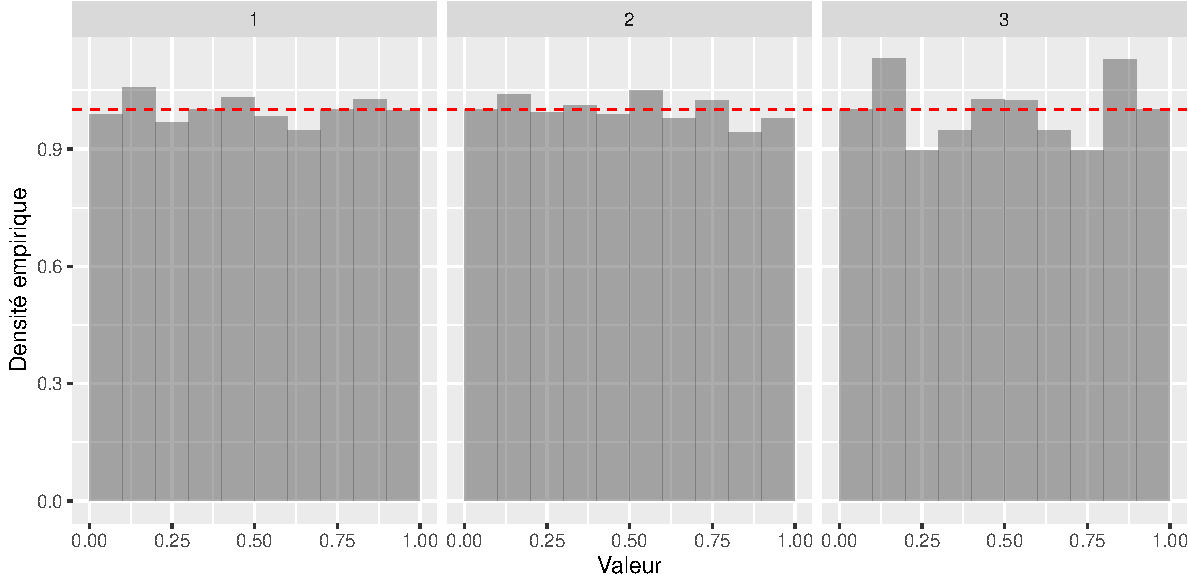
\includegraphics{correction_simulation_variables_aleatoires_files/figure-latex/histogramme1-1} \end{center}

\textbackslash{}begin\{Correction\}

Les deux échantillons ont l'air de couvrir à peu près uniformément
l'intervalle {[}0, 1{]}. Le 3ème par contre semble poser problème. On
peut regarder le résultats du test d'adéquation de Kolmogorov Smirnoff.
On ne regarde ici que les probabilités critiques du test (effectués par
numéro, d'où le \textbackslash{}texttt\{group\_by\} avec la fonction
\texttt{ks.test}).

\textbackslash{}end\{Correction\}

\begin{Shaded}
\begin{Highlighting}[]
\NormalTok{kolmog_smirnoff_test_p_values <-}\StringTok{ }\NormalTok{resultats }\OperatorTok
\StringTok{  }\KeywordTok{group_by}\NormalTok{(generateur) }\OperatorTok\StringTok{ }\CommentTok{# On regroupe les genrateurs ensembles}
\StringTok{  }\CommentTok{# pour chaque generateur, on effectue le test de kolmogoroff smirnoff}
\StringTok{  }\CommentTok{# on extrait la p valeur et on la stocke dans p_val}
\StringTok{  }\KeywordTok{summarise}\NormalTok{(}\DataTypeTok{p_val =} \KeywordTok{ks.test}\NormalTok{(u, }\DataTypeTok{y =} \StringTok{"punif"}\NormalTok{)}\OperatorTok{$}\NormalTok{p.value)}
\NormalTok{kolmog_smirnoff_test_p_values}
\end{Highlighting}
\end{Shaded}

\begin{verbatim}
# A tibble: 3 x 2
  generateur   p_val
  <chr>        <dbl>
1 1          0.757  
2 2          0.294  
3 3          0.00251
\end{verbatim}

\begin{Correction}

Au risque de première espèce $\alpha = 1\%$, on rejette $H_0$ pour le troisième générateur.

\end{Correction}

\begin{enumerate}
\def\labelenumi{\arabic{enumi}.}
\setcounter{enumi}{3}
\tightlist
\item
  Pour chacun des échantillons \((u_1,\dots, u_{10000})\) obtenus,
  tracez \(u_n\) en fonction de \(u_{n-1}\). Que pouvez vous conclure
  sur la qualité des 3 générateurs?
\end{enumerate}

\begin{Shaded}
\begin{Highlighting}[]
\NormalTok{resultats }\OperatorTok
\StringTok{  }\KeywordTok{group_by}\NormalTok{(generateur) }\OperatorTok
\StringTok{  }\CommentTok{# Pour chaque generateur, on cree une colonne u_n_plus1  comprenant u[n+1]}
\StringTok{  }\KeywordTok{mutate}\NormalTok{(}\DataTypeTok{u_n_plus1 =} \KeywordTok{lead}\NormalTok{(u)) }\OperatorTok\StringTok{ }\CommentTok{# mutate est une fonction de creation de colonne}
\StringTok{  }\KeywordTok{ggplot}\NormalTok{() }\OperatorTok{+}\StringTok{ }\CommentTok{# on représente graphiquement le resultat}
\StringTok{  }\KeywordTok{aes}\NormalTok{(}\DataTypeTok{x =}\NormalTok{ u, }\DataTypeTok{y =}\NormalTok{ u_n_plus1) }\OperatorTok{+}\StringTok{ }\CommentTok{# u[n+1] en fonction de u[n]}
\StringTok{  }\KeywordTok{geom_point}\NormalTok{() }\OperatorTok{+}\StringTok{ }\CommentTok{# On représente un point par couple}
\StringTok{  }\KeywordTok{facet_wrap}\NormalTok{(.}\OperatorTok{~}\NormalTok{generateur) }\OperatorTok{+}\StringTok{ }\CommentTok{# Un graphe par generateur}
\StringTok{  }\KeywordTok{labs}\NormalTok{(}\DataTypeTok{x =} \KeywordTok{expression}\NormalTok{(u[n]), }\DataTypeTok{y =} \KeywordTok{expression}\NormalTok{(u[n }\OperatorTok{+}\StringTok{ }\DecValTok{1}\NormalTok{])) }\CommentTok{# Habillage}
\end{Highlighting}
\end{Shaded}

\begin{center}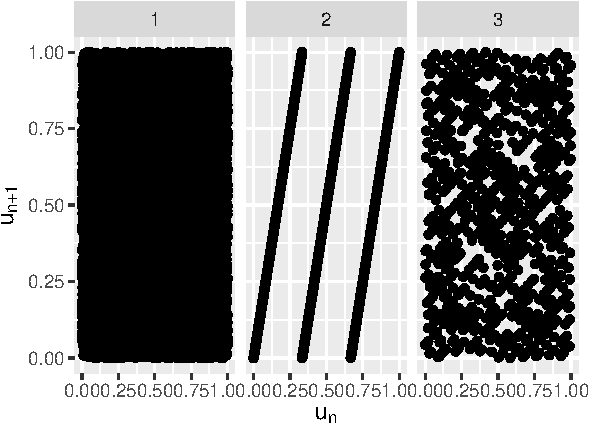
\includegraphics{correction_simulation_variables_aleatoires_files/figure-latex/plots_autocorrelation-1} \end{center}

\hypertarget{muxe9thode-dinversion}{%
\section{Méthode d'inversion}\label{muxe9thode-dinversion}}

\hypertarget{loi-exponentielle}{%
\subsection{Loi exponentielle}\label{loi-exponentielle}}

On rappelle qu'une variable aléatoire \(X\) est de loi exponentielle de
paramètre \(\lambda > 0\) si elle a pour fonction de densité
\(f_X(x) = \lambda\text{e}^{-\lambda x} \mathbf{1}_{x\geq0}\)

\begin{enumerate}
\def\labelenumi{\arabic{enumi}.}
\tightlist
\item
  En utilisant la méthode d'inversion, proposez un algorithme de
  simulation pour une variable aléatoire exponentielle.
\end{enumerate}

\begin{Correction}

On a que
\begin{align*}
F(x) &= \int_\mathbb{-\infty}^x \lambda\text{e}^{-\lambda z} \mathbf{1}_{z\geq0} dz\\
&= 1 - \text{e}^{-\lambda x}
\end{align*}
Cette fonction est continue et bijective de $\mathbb{R^+}$ dans $]0,1[$, son inverse est, pour $u\in ]0, 1[$
$$F^{-1}(u) = -\frac{\ln (1 - u)}{\lambda}$$

Ainsi, si on simule une variable aléatoire $U\sim \mathcal{U}[0, 1]$, alors
$X = -\frac{\ln (1 - U)}{\lambda}$ est distribuée selon une variable aléatoire exponentielle de
paramètre $\lambda$.

\end{Correction}

\begin{enumerate}
\def\labelenumi{\arabic{enumi}.}
\setcounter{enumi}{1}
\tightlist
\item
  Ecrire une fonction \texttt{R} mettant en oeuvre cette algorithme.
  Cette fonction prendra deux paramètres en entrée:
\end{enumerate}

\begin{itemize}
\tightlist
\item
  \texttt{n} La taille de l'échantillon;
\item
  \texttt{lambda} Le paramètre de la loi exponentielle
\end{itemize}

Vous testerez la qualité de votre fonction sur un échantillon de taille
10000, en comparant graphiquement l'histogramme empirique obtenu à la
densité de la loi exponentielle correspondante.

\begin{Shaded}
\begin{Highlighting}[]
\NormalTok{mon_rexp <-}\StringTok{ }\ControlFlowTok{function}\NormalTok{(n, lambda)\{}
\NormalTok{  us <-}\StringTok{ }\KeywordTok{runif}\NormalTok{(n)}\CommentTok{# Vecteur d'uniformes}
\NormalTok{  echantillon =}\StringTok{ }\OperatorTok{-}\StringTok{ }\KeywordTok{log}\NormalTok{(}\DecValTok{1} \OperatorTok{-}\StringTok{ }\NormalTok{us) }\OperatorTok{/}\StringTok{ }\NormalTok{lambda}
  \KeywordTok{return}\NormalTok{(}\KeywordTok{tibble}\NormalTok{(}\DataTypeTok{n =} \DecValTok{1}\OperatorTok{:}\NormalTok{n, }\DataTypeTok{valeur =}\NormalTok{ echantillon))}
\NormalTok{\}}
\end{Highlighting}
\end{Shaded}

\begin{Correction}

On simule un échantillon, et on en trace le graphe

\end{Correction}

\begin{Shaded}
\begin{Highlighting}[]
\KeywordTok{set.seed}\NormalTok{(}\DecValTok{123}\NormalTok{)}\CommentTok{# Fixe la graine aléatoire dans runif, pour reproductibilité}
\NormalTok{lambda <-}\StringTok{ }\DecValTok{1}
\NormalTok{echantillon_exp <-}\StringTok{ }\KeywordTok{mon_rexp}\NormalTok{(}\FloatTok{1e4}\NormalTok{, lambda)}
\NormalTok{my_breaks <-}\StringTok{ }\KeywordTok{seq}\NormalTok{(}\DecValTok{0}\NormalTok{, }\DecValTok{10}\NormalTok{, }\DataTypeTok{by =} \FloatTok{0.1}\NormalTok{)}\CommentTok{# Point de ruptures de l'histogramme}
\KeywordTok{ggplot}\NormalTok{(echantillon_exp,  }\DataTypeTok{mapping =} \KeywordTok{aes}\NormalTok{(}\DataTypeTok{x =}\NormalTok{ valeur)) }\OperatorTok{+}
\StringTok{  }\KeywordTok{geom_histogram}\NormalTok{(}\DataTypeTok{mapping =} \KeywordTok{aes}\NormalTok{(}\DataTypeTok{y =}\NormalTok{ ..density..), }\DataTypeTok{fill =} \StringTok{"lightblue"}\NormalTok{,}
                 \DataTypeTok{breaks =}\NormalTok{ my_breaks) }\OperatorTok{+}
\StringTok{  }\KeywordTok{geom_line}\NormalTok{(}\DataTypeTok{data =} \KeywordTok{data.frame}\NormalTok{(}\DataTypeTok{x =}\NormalTok{ my_breaks, }\DataTypeTok{y =} \KeywordTok{dexp}\NormalTok{(my_breaks, lambda)),}
            \DataTypeTok{mapping =} \KeywordTok{aes}\NormalTok{(}\DataTypeTok{x =}\NormalTok{ x, }\DataTypeTok{y=}\NormalTok{ y), }\DataTypeTok{col =} \StringTok{"red"}\NormalTok{) }\OperatorTok{+}
\StringTok{  }\KeywordTok{theme_bw}\NormalTok{() }\OperatorTok{+}\StringTok{ }\KeywordTok{labs}\NormalTok{(}\DataTypeTok{x =} \StringTok{"X"}\NormalTok{, }\DataTypeTok{y =} \StringTok{"Densité"}\NormalTok{, }\DataTypeTok{title =} \StringTok{"Histogramme empirique"}\NormalTok{)}
\end{Highlighting}
\end{Shaded}

\begin{center}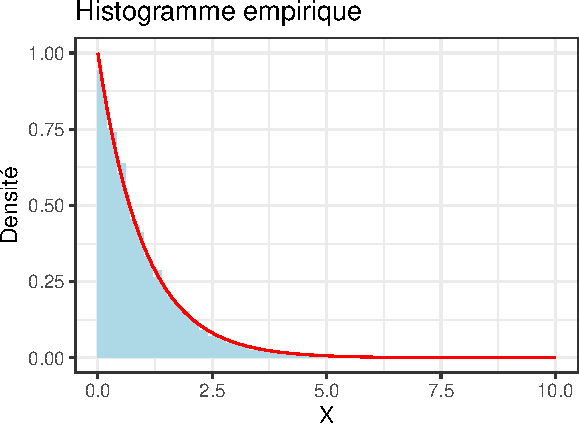
\includegraphics{correction_simulation_variables_aleatoires_files/figure-latex/plot_echantillon_mon_rexp-1} \end{center}

\hypertarget{loi-discruxe8te}{%
\subsection{Loi discrète}\label{loi-discruxe8te}}

\label{exo:inv:disc} On considère une variable aléatoire discrète \(X\)
à valeurs dans l'ensemble \(\left\lbrace 1,\dots, K\right\rbrace\), dont
la loi est définie par le vecteur de probabilité \((p_1, \dots, p_K)\),
i.e.: \begin{align}
\mathbb{P}(X = k) &= p_k\\
\sum_{k = 1}^K p_k &= 1
\end{align}

\begin{enumerate}
\def\labelenumi{\arabic{enumi}.}
\tightlist
\item
  Pour tout \(u \in ]0, 1[\), écrire l'expression de l'inverse
  généralisée de la fonction de répartition de \(X\).
\end{enumerate}

\begin{Correction}

$$F(x) = \sum_{k = 1}^{K}p_k\mathbf{1}_{k \leq x}$$
$$F^{-1}(u) = \left\lbrace
\begin{array}{lcr}
1 &si&0 < u \leq p_1\\
2 &si&p_1 < u \leq p_1 + p_2\\
\dots & & \dots\\
k &si &\sum_{i = 1}^{k - 1} p_i < u \leq \sum_{i = 1}^{k} p_i\\
\dots & & \dots\\
K&si& \sum_{i = 1}^{K - 1} p_i < u < 1
\end{array}
\right.$$

\end{Correction}

\begin{enumerate}
\def\labelenumi{\arabic{enumi}.}
\setcounter{enumi}{1}
\tightlist
\item
  En déduire un algorithme de simulation pour toute variable aléatoire
  discrète dans un ensemble fini.
\end{enumerate}

\begin{Correction}

Ainsi, il suffit de tirer $U\sim \mathcal{U}[0, 1]$ et de trouver l'indice $k$ tel que $\sum_{i = 1}^{k - 1} p_i < u \leq \sum_{i = 1}^{k} p_i$

\end{Correction}

\begin{enumerate}
\def\labelenumi{\arabic{enumi}.}
\setcounter{enumi}{2}
\tightlist
\item
  Utilisez cet algorithme de simulation pour simuler un échantillon de
  taille 10000 loi binomiale de paramètres \(n = 10\) et \(p = 0.5\)
  avec \texttt{R}. Vous comparerez les fréquences obtenues avec les
  fréquences théoriques.
\end{enumerate}

\begin{Correction}

On utilisera \texttt{dbinom} pour calculer les probabilités d'une loi binomiale.
Ensuite, la fonction findInterval évite de faire une boucle.

\end{Correction}

\begin{Shaded}
\begin{Highlighting}[]
\NormalTok{mon_rbinom <-}\StringTok{ }\ControlFlowTok{function}\NormalTok{(n, n_binom, p)\{}
  \CommentTok{# Pour les probas on utilise la fonction dbinom}
\NormalTok{  (vecteur_probs <-}\StringTok{ }\KeywordTok{c}\NormalTok{(}\DecValTok{0}\NormalTok{, }\KeywordTok{dbinom}\NormalTok{(}\DecValTok{0}\OperatorTok{:}\NormalTok{n_binom, }\DataTypeTok{size =}\NormalTok{ n_binom, }\DataTypeTok{prob =}\NormalTok{ p)))}
\NormalTok{  (prob_cumule <-}\StringTok{ }\KeywordTok{cumsum}\NormalTok{(vecteur_probs)) }\CommentTok{# Probas cumules)}
\NormalTok{  us <-}\StringTok{ }\KeywordTok{runif}\NormalTok{(n)}
  \CommentTok{# La fonction findInterval permet de trouver dans quel intervalle se trouve}
  \CommentTok{# un u}
\NormalTok{  intervalles <-}\StringTok{ }\KeywordTok{findInterval}\NormalTok{(us, prob_cumule, }\DataTypeTok{rightmost.closed =}\NormalTok{ T,}
                              \DataTypeTok{left.open =}\NormalTok{ T)}
  \CommentTok{# Il faut retrancher 1 à "intervalles" pour obtenir les valeurs attendues}
  \CommentTok{# d'une binomiale}
  \KeywordTok{return}\NormalTok{(}\KeywordTok{data.frame}\NormalTok{(}\DataTypeTok{n =} \DecValTok{1}\OperatorTok{:}\NormalTok{n,}
                    \DataTypeTok{valeur =} \KeywordTok{factor}\NormalTok{(intervalles }\OperatorTok{-}\StringTok{ }\DecValTok{1}\NormalTok{, }\DataTypeTok{levels =} \DecValTok{0}\OperatorTok{:}\NormalTok{n_binom)))}
\NormalTok{\}}
\end{Highlighting}
\end{Shaded}

\begin{Shaded}
\begin{Highlighting}[]
\CommentTok{# Représentation graphique}
\KeywordTok{set.seed}\NormalTok{(}\DecValTok{123}\NormalTok{) }\CommentTok{# Pour la reproductibilité}
\NormalTok{n_sample <-}\StringTok{ }\FloatTok{1e4}\NormalTok{; n_binom <-}\StringTok{ }\DecValTok{10}\NormalTok{; p <-}\StringTok{ }\FloatTok{0.5} \CommentTok{# Parametre}
\NormalTok{echantillon_binom <-}\StringTok{ }\KeywordTok{mon_rbinom}\NormalTok{(n_sample, n_binom, p) }\CommentTok{# Echantillon génére}
\end{Highlighting}
\end{Shaded}

\begin{Shaded}
\begin{Highlighting}[]
\CommentTok{# Calcul et stockage des fréquences empiriques}
\NormalTok{frequences_empiriques <-}\StringTok{ }\NormalTok{echantillon_binom }\OperatorTok\StringTok{ }
\StringTok{  }\KeywordTok{group_by}\NormalTok{(valeur, }\DataTypeTok{.drop =} \OtherTok{FALSE}\NormalTok{) }\OperatorTok\StringTok{ }\CommentTok{# On regroupe par valeur de nbre de succes}
\StringTok{  }\KeywordTok{summarise}\NormalTok{(}\DataTypeTok{freq_empir =} \KeywordTok{n}\NormalTok{() }\OperatorTok{/}\StringTok{ }\NormalTok{n_sample) }\OperatorTok\StringTok{ }\CommentTok{# On divise le nombre total n() par n_sample}
\StringTok{  }\KeywordTok{ungroup}\NormalTok{() }\OperatorTok\StringTok{ }\CommentTok{# On dégroupe}
\StringTok{  }\KeywordTok{mutate}\NormalTok{(}\DataTypeTok{freq_theo =} \KeywordTok{dbinom}\NormalTok{(}\DecValTok{0}\OperatorTok{:}\NormalTok{n_binom, n_binom, p)) }\CommentTok{# On ajoute la fréquence theorique}
\end{Highlighting}
\end{Shaded}

\begin{Shaded}
\begin{Highlighting}[]
\CommentTok{# Représentation graphique}
\KeywordTok{ggplot}\NormalTok{(frequences_empiriques) }\OperatorTok{+}\StringTok{ }\CommentTok{# Tableau à représenter}
\StringTok{  }\KeywordTok{aes}\NormalTok{(}\DataTypeTok{x =}\NormalTok{ valeur) }\OperatorTok{+}\StringTok{ }\CommentTok{# Abscisse commune}
\StringTok{  }\KeywordTok{geom_col}\NormalTok{(}\DataTypeTok{mapping =} \KeywordTok{aes}\NormalTok{(}\DataTypeTok{y =}\NormalTok{ freq_empir), }\CommentTok{# Ordonnée des fréquences empiriques}
           \DataTypeTok{width =} \FloatTok{0.2}\NormalTok{, }\DataTypeTok{fill =} \StringTok{"lightblue"}\NormalTok{) }\OperatorTok{+}
\StringTok{  }\KeywordTok{geom_point}\NormalTok{(}\KeywordTok{aes}\NormalTok{(}\DataTypeTok{y =}\NormalTok{ freq_theo), }\CommentTok{# On ajoute le point des fréquences théoriques }
             \DataTypeTok{shape =} \DecValTok{3}\NormalTok{, }\DataTypeTok{col =} \StringTok{"red"}\NormalTok{, }\DataTypeTok{size =} \DecValTok{3}\NormalTok{) }\OperatorTok{+}
\StringTok{  }\KeywordTok{labs}\NormalTok{(}\DataTypeTok{y =} \StringTok{"Fréquence"}\NormalTok{, }\DataTypeTok{x =} \StringTok{"Nombre de succès"}\NormalTok{)}
\end{Highlighting}
\end{Shaded}

\begin{center}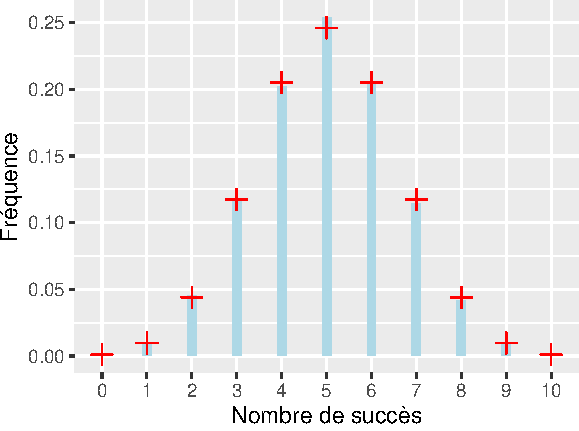
\includegraphics{correction_simulation_variables_aleatoires_files/figure-latex/plot_frequences_empiriques-1} \end{center}

\hypertarget{muxe9thode-de-rejet}{%
\section{Méthode de rejet}\label{muxe9thode-de-rejet}}

\hypertarget{simulation-dune-loi-de-poisson-pour-lambda-1}{%
\subsection{\texorpdfstring{Simulation d'une loi de Poisson pour
\(\lambda < 1\)}{Simulation d'une loi de Poisson pour \textbackslash{}lambda \textless{} 1}}\label{simulation-dune-loi-de-poisson-pour-lambda-1}}

\begin{enumerate}
\def\labelenumi{\arabic{enumi}.}
\tightlist
\item
  On utilisant le résultat de l'exercice \ref{exo:inv:disc}, proposez un
  algorithme pour simuler une variable aléatoire de Bernouilli de
  paramètre \(p \in ]0, 1[\).
\end{enumerate}

\begin{Correction}

Il suffit de tirer une uniforme $U$, et de poser $X = 0$ si $U \leq 1 - p$, 1 sinon.

\end{Correction}

\begin{enumerate}
\def\labelenumi{\arabic{enumi}.}
\setcounter{enumi}{1}
\tightlist
\item
  En déduire un algorithme pour simuler une loi géométrique de paramètre
  \(p\) sur \(\mathbb{N}\).
\end{enumerate}

\begin{Correction}

Une variable aléatoire $Y$ de loi géométrique sur $\mathbb{N}$  de paramètre $p$ est la loi du nombre d'échecs d'une Bernouilli de paramètre $p$ avant le premier succès.

Ainsi, on initialise à $Y = 0$, et on simule $X$. Tant que $X = 0$, on pose $Y = Y +1$.

\end{Correction}

\begin{enumerate}
\def\labelenumi{\arabic{enumi}.}
\setcounter{enumi}{2}
\tightlist
\item
  On souhaite obtenir un échantillon d'une loi de de Poisson de
  paramètre \(\lambda \in ]0, 1[\) par méthode d'acceptation rejet. On
  se propose d'utiliser comme loi de proposition la loi géométrique sur
  \(\mathbb{N}\) de paramètre \(1 - \lambda\). Définir l'algorithme de
  rejet correspondant.
\end{enumerate}

\begin{Correction}

On veut simuler selon $Z$, une variable aléatoire de loi de poisson  de paramètre $\lambda \in ]0, 1[$. On prend comme loi de proposition la loi géométrique sur $\mathbb{N}$ de paramètre $(1 - \lambda)$. On note $Y$ une variable aléatoire de cette loi.
Pour $k \in \mathbb{N}$, on a:

\begin{align*}
\mathbb{P}(Z = k) &= \frac{\lambda^k}{k!}\text{e}^{-\lambda}\\
\mathbb{P}(Y = k) &= \lambda^{k}(1 - \lambda)
\end{align*}
On a:
\begin{align*}
\frac{\mathbb{P}(Z = k)}{\mathbb{P}(Y = k)} &= \frac{\text{e}^{-\lambda}}{k! (1 - \lambda)}\\
&\leq \frac{\text{e}^{-\lambda}}{(1 - \lambda)} : = M
\end{align*}

Ainsi, pour simuler une réalisation $z$ selon $Z$, on a l'algorithme suivant:

\begin{enumerate}
\item Simuler une réalisation $y$ d'une loi géométrique  de paramètre $p = 1 - \lambda$.
\item Simuler une loi uniforme $u$ sur [0, 1].
\item $$u \leq \frac{\mathbb{P}(Z = y)}{M\mathbb{P}(Y = y)},$$ poser $z = y$, sinon, retourner en 1.
\end{enumerate}

\end{Correction}

\begin{enumerate}
\def\labelenumi{\arabic{enumi}.}
\setcounter{enumi}{3}
\tightlist
\item
  Quelle est la probabilité d'acceptation dans l'algorithme de rejet?
\end{enumerate}

\begin{Correction}
La probabilité d'acceptation dans l'algorithme de rejet est donnée par
$\frac{1 - \lambda}{e^{-\lambda}}$, qui tend vers 0 quand $\lambda$ tend vers 1.
\end{Correction}

\begin{enumerate}
\def\labelenumi{\arabic{enumi}.}
\setcounter{enumi}{4}
\tightlist
\item
  Faites une fonction \texttt{R} permettant de générer une loi
  géométrique de paramètre \(p\). Utiliser cette fonction dans une autre
  fonction \texttt{R} permettant de simuler selon une loi de Poisson de
  paramètre \(p \in ]0, 1[\). Simuler ainsi un échantillon de taille
  10000. Comparer la distribution obtenue à celle de la vraie loi.
\end{enumerate}

\begin{Shaded}
\begin{Highlighting}[]
\CommentTok{# Simulation d'une bernouilli}
\NormalTok{mon_rbern <-}\StringTok{ }\ControlFlowTok{function}\NormalTok{(n, p)\{}
\NormalTok{  us <-}\StringTok{ }\KeywordTok{runif}\NormalTok{(n) }\CommentTok{# Echantillon uniforme}
  \KeywordTok{ifelse}\NormalTok{(}\DataTypeTok{test =}\NormalTok{ us }\OperatorTok{<}\StringTok{ }\DecValTok{1} \OperatorTok{-}\StringTok{ }\NormalTok{p, }\CommentTok{# Pour chaque u, on checke si u < 1- p}
         \DataTypeTok{yes =} \DecValTok{0}\NormalTok{, }\CommentTok{# Si oui, on assigne la valeur 0}
         \DataTypeTok{no =} \DecValTok{1}\NormalTok{)  }\CommentTok{# Si non la valeur 1}
\NormalTok{\}}
\end{Highlighting}
\end{Shaded}

\begin{Shaded}
\begin{Highlighting}[]
\CommentTok{# On peut donc coder la fonction rgeom qui simule une loi géométrique}
\CommentTok{# (défini comme le nombre d'échecs avant le 1er succès)}
\NormalTok{mon_rgeom <-}\StringTok{ }\ControlFlowTok{function}\NormalTok{(n, p)\{}
\NormalTok{  get_one_sample <-}\StringTok{ }\ControlFlowTok{function}\NormalTok{()\{}\CommentTok{# On fait la fonction (en interne) pour 1 simu}
\NormalTok{    nb_echecs <-}\StringTok{ }\DecValTok{-1} \CommentTok{# Nombre d'échecs courant (initialisé à - 1)}
\NormalTok{    stopping_condition <-}\StringTok{ }\OtherTok{FALSE}
    \ControlFlowTok{while}\NormalTok{(}\OperatorTok{!}\NormalTok{stopping_condition)\{}
\NormalTok{      nb_echecs <-}\StringTok{ }\NormalTok{nb_echecs }\OperatorTok{+}\StringTok{ }\DecValTok{1} \CommentTok{# Le nombre d'échecs augmente}
\NormalTok{      bernouilli_sample <-}\StringTok{  }\KeywordTok{mon_rbern}\NormalTok{(}\DecValTok{1}\NormalTok{, p) }\CommentTok{# Simulation d'un Bernouilli}
\NormalTok{      stopping_condition <-}\StringTok{ }\NormalTok{bernouilli_sample }\OperatorTok{==}\StringTok{ }\DecValTok{1} \CommentTok{# Condition d'arret}
\NormalTok{    \}}
    \KeywordTok{return}\NormalTok{(nb_echecs)}
\NormalTok{  \} }
  \CommentTok{# On reproduit n fois le même traitement grâce à rerun}
  \KeywordTok{rerun}\NormalTok{(n, }
        \KeywordTok{get_one_sample}\NormalTok{()) }\OperatorTok\StringTok{ }\CommentTok{# Renvoit une liste}
\StringTok{    }\KeywordTok{unlist}\NormalTok{()  }\CommentTok{# Le resultat final est un vecteur}
\NormalTok{\}}
\end{Highlighting}
\end{Shaded}

\begin{Shaded}
\begin{Highlighting}[]
\CommentTok{# On se sert de cette fonction pour simuler une loi de poisson}
\NormalTok{mon_rpois <-}\StringTok{ }\ControlFlowTok{function}\NormalTok{(n, lambda) \{}
  \ControlFlowTok{if}\NormalTok{ (lambda }\OperatorTok{>=}\StringTok{ }\DecValTok{1} \OperatorTok{|}\StringTok{ }\NormalTok{lambda }\OperatorTok{<=}\StringTok{ }\DecValTok{0}\NormalTok{) \{}
    \KeywordTok{stop}\NormalTok{(}\StringTok{"In this function, lambda must be between 0 and 1"}\NormalTok{)}
\NormalTok{  \}}
\NormalTok{  M <-}\StringTok{ }\KeywordTok{exp}\NormalTok{(}\OperatorTok{-}\NormalTok{lambda) }\OperatorTok{/}\StringTok{ }\NormalTok{(}\DecValTok{1} \OperatorTok{-}\StringTok{ }\NormalTok{lambda) }\CommentTok{# Borne uniforme}
\NormalTok{  get_one_sample <-}\StringTok{ }\ControlFlowTok{function}\NormalTok{()\{ }\CommentTok{# Fonction de génération d'un individu}
\NormalTok{    accepted <-}\StringTok{ }\OtherTok{FALSE} \CommentTok{# A t'on accepte un candidat?}
    \ControlFlowTok{while}\NormalTok{(}\OperatorTok{!}\NormalTok{accepted)\{}
\NormalTok{      candidate <-}\StringTok{ }\KeywordTok{mon_rgeom}\NormalTok{(}\DecValTok{1}\NormalTok{, }\DecValTok{1} \OperatorTok{-}\StringTok{ }\NormalTok{lambda) }\CommentTok{# Simule selon une géométrique}
      \CommentTok{# ratio d'acceptation}
      \CommentTok{# dpois et dgeom donnent les lois de poisson et geometrique (sur N) dans R}
\NormalTok{      ratio <-}\StringTok{ }\KeywordTok{dpois}\NormalTok{(candidate, lambda) }\OperatorTok{/}\StringTok{ }\NormalTok{(M }\OperatorTok{*}\StringTok{ }\KeywordTok{dgeom}\NormalTok{(candidate, }\DecValTok{1} \OperatorTok{-}\StringTok{ }\NormalTok{lambda))}
\NormalTok{      u <-}\StringTok{ }\KeywordTok{runif}\NormalTok{(}\DecValTok{1}\NormalTok{, }\DataTypeTok{min =} \DecValTok{0}\NormalTok{, }\DataTypeTok{max =} \DecValTok{1}\NormalTok{)}
\NormalTok{      accepted <-}\StringTok{ }\NormalTok{(u }\OperatorTok{<=}\StringTok{ }\NormalTok{ratio)}\CommentTok{# A t'on accepté?}
\NormalTok{    \}}
    \KeywordTok{return}\NormalTok{(candidate)}
\NormalTok{  \}}
  \KeywordTok{rerun}\NormalTok{(n, }\CommentTok{# Rerun n times the get_one_sample function}
               \KeywordTok{get_one_sample}\NormalTok{()) }\OperatorTok\StringTok{ }\CommentTok{# returns a list}
\StringTok{    }\KeywordTok{unlist}\NormalTok{() }\OperatorTok\StringTok{ }\CommentTok{# Transformed into a vector}
\StringTok{    }\KeywordTok{tibble}\NormalTok{(}\DataTypeTok{n =} \DecValTok{1}\OperatorTok{:}\NormalTok{n, }\DataTypeTok{x =}\NormalTok{ .) }\CommentTok{# Put into a tibble to ease ggplots}
\NormalTok{\}}
\end{Highlighting}
\end{Shaded}

\begin{Shaded}
\begin{Highlighting}[]
\KeywordTok{set.seed}\NormalTok{(}\DecValTok{123}\NormalTok{)}\CommentTok{# Manière de "fixer" l'aléa (pour des résultats reproductibles)}
\NormalTok{n_sample <-}\StringTok{ }\FloatTok{1e4}
\NormalTok{lambda <-}\StringTok{ }\FloatTok{0.5}
\NormalTok{poisson_sample <-}\StringTok{ }\KeywordTok{mon_rpois}\NormalTok{(n_sample, lambda)}
\end{Highlighting}
\end{Shaded}

\begin{Correction}
Pour la représentation graphique, on commence par extraire les fréquences empiriques et les fréquences théoriques.
\end{Correction}

\begin{Shaded}
\begin{Highlighting}[]
\CommentTok{# On représente l'histogramme empirique jusqu'à k_ma, le maximum observé}
\CommentTok{# dans l'échantillon}
\NormalTok{k_max <-}\StringTok{ }\KeywordTok{max}\NormalTok{(poisson_sample}\OperatorTok{$}\NormalTok{x)}
\NormalTok{frequences <-}\StringTok{ }\NormalTok{poisson_sample }\OperatorTok\StringTok{ }
\StringTok{  }\KeywordTok{mutate}\NormalTok{(}\DataTypeTok{x =} \KeywordTok{factor}\NormalTok{(x, }\DataTypeTok{levels =} \DecValTok{0}\OperatorTok{:}\NormalTok{k_max)) }\OperatorTok\StringTok{ }\CommentTok{# On transforme en facteur}
\StringTok{  }\KeywordTok{group_by}\NormalTok{(x) }\OperatorTok\StringTok{ }
\StringTok{  }\KeywordTok{summarise}\NormalTok{(}\DataTypeTok{freq_empir =} \KeywordTok{n}\NormalTok{() }\OperatorTok{/}\StringTok{ }\NormalTok{n_sample) }\OperatorTok\StringTok{ }
\StringTok{  }\KeywordTok{ungroup}\NormalTok{() }\OperatorTok\StringTok{ }
\StringTok{  }\KeywordTok{mutate}\NormalTok{(}\DataTypeTok{freq_theo =} \KeywordTok{dpois}\NormalTok{(}\DecValTok{0}\OperatorTok{:}\NormalTok{k_max, lambda))}
\end{Highlighting}
\end{Shaded}

\begin{Shaded}
\begin{Highlighting}[]
\NormalTok{frequences }\OperatorTok\StringTok{ }\CommentTok{# On transforme légèrement pour le graphique}
\StringTok{  }\KeywordTok{gather}\NormalTok{(}\OperatorTok{-}\NormalTok{x, }\DataTypeTok{key =} \StringTok{"Distribution"}\NormalTok{, }\DataTypeTok{value =} \StringTok{"Proba"}\NormalTok{) }\OperatorTok\StringTok{ }\CommentTok{# Regardez ce que ca fait!}
\StringTok{  }\KeywordTok{ggplot}\NormalTok{() }\OperatorTok{+}\StringTok{ }\CommentTok{# on représente le résultat}
\StringTok{  }\KeywordTok{aes}\NormalTok{(}\DataTypeTok{x =}\NormalTok{ x, }\DataTypeTok{y =}\NormalTok{ Proba) }\OperatorTok{+}\StringTok{ }\CommentTok{# }
\StringTok{  }\KeywordTok{geom_col}\NormalTok{(}\DataTypeTok{mapping =} \KeywordTok{aes}\NormalTok{(}\DataTypeTok{fill =}\NormalTok{ Distribution), }\CommentTok{# Ordonnée des fréquences empiriques}
           \DataTypeTok{width =} \FloatTok{0.3}\NormalTok{, }\DataTypeTok{position =} \StringTok{"dodge"}\NormalTok{) }\OperatorTok{+}
\StringTok{  }\KeywordTok{labs}\NormalTok{(}\DataTypeTok{x =} \StringTok{"k"}\NormalTok{, }\DataTypeTok{y =} \StringTok{"Probabilité"}\NormalTok{) }\OperatorTok{+}
\StringTok{  }\KeywordTok{scale_fill_discrete}\NormalTok{(}\DataTypeTok{labels =} \KeywordTok{c}\NormalTok{(}\StringTok{"Empirique"}\NormalTok{, }\StringTok{"Théorique"}\NormalTok{))}
\end{Highlighting}
\end{Shaded}

\begin{center}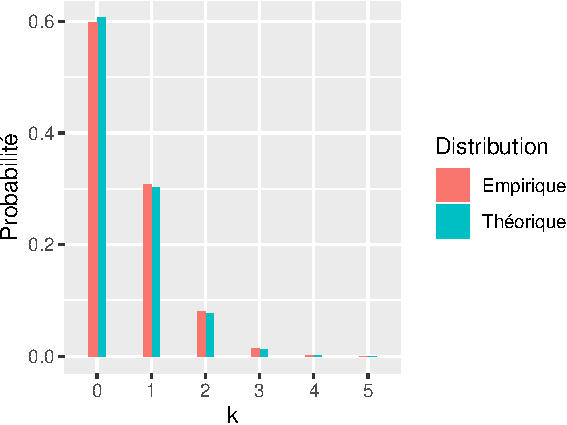
\includegraphics{correction_simulation_variables_aleatoires_files/figure-latex/plot_frequences_poisson-1} \end{center}

\hypertarget{loi-uniforme-sur-le-disque-unituxe9}{%
\subsection{Loi uniforme sur le disque
unité}\label{loi-uniforme-sur-le-disque-unituxe9}}

\begin{enumerate}
\def\labelenumi{\arabic{enumi}.}
\tightlist
\item
  À partir d'une variable aléatoire uniforme sur \([0, 1]\), proposez
  une transformation pour simuler une loi uniforme sur \([-1, 1]\).
\end{enumerate}

\begin{Correction}
Si U est une uniforme sur [0,1], alors, la variable aléatoire $2U - 1$ est une uniforme
sur [-1, 1]
\end{Correction}

\begin{enumerate}
\def\labelenumi{\arabic{enumi}.}
\setcounter{enumi}{1}
\tightlist
\item
  Proposer une méthode d'acceptation rejet pour simuler, à partir de
  deux variables aléatoires indépendantes de loi uniforme sur
  \([-1, 1]\), une variable aléatoire uniforme sur le disque unité.
\end{enumerate}

\begin{Correction}
Un point $(x, y)$ de $\mathbb{R^2}$ est dans le disque unité si $x^2 + y^2 \leq 1$.
L'aire de cette surface est de $\pi$.

La densité de la loi uniforme sur le disque unité est donc
$$f_D(x, y) = \frac{\mathbf{1}_{x^2 + y^2 \leq 1}}{\pi}$$

La densité de la loi uniforme sur le carré de $[-1, 1] \times [-1, 1]$ est
$$g_C(x, y) = \frac{\mathbf{1}_{-1\leq x \leq 1} \mathbf{1}_{-1 \leq y\leq 1}}{4}$$
On ainsi que pour tout $(x, y)$ $f_D(x, y) \leq \frac{4}{\pi} g_C(x, y)$.

Le ratio d'acceptation est donc simplement
$$\alpha(x, y) = \frac{\pi}{4}\frac{f_D(x, y)}{g_C(x, y)} = \frac{\mathbf{1}_{x^2 + y^2 \leq 1}}{\mathbf{1}_{-1\leq x \leq 1} \mathbf{1}_{-1 \leq y\leq 1}}$$

L'algorithme est donc:

\begin{enumerate}
\item On simule 2 uniformes $U$ et $V$ sur [-1, 1] indépendamment.
\item On accepte le couple $U$, $V$ si il tombe dans le disque unité (i.e. $U^2 + V^2 \leq 1$), on recommence sinon
\end{enumerate}

\end{Correction}

\begin{enumerate}
\def\labelenumi{\arabic{enumi}.}
\setcounter{enumi}{2}
\tightlist
\item
  Quelle est la probabilité d'acceptation de l'algorithme?
\end{enumerate}

\begin{Correction}
La probabilité d'acceptation de l'algorithme est donc de $\frac{\pi}{4}$
\end{Correction}

\begin{enumerate}
\def\labelenumi{\arabic{enumi}.}
\setcounter{enumi}{3}
\tightlist
\item
  Ecrire une fonction \texttt{R} mettant en place la génération de
  variables aléatoires sur le disque unité. Dans cet algorithme, gardez
  en mémoire le nombre d'essais nécessaire avant chaque acceptation.
\end{enumerate}

\begin{Shaded}
\begin{Highlighting}[]
\NormalTok{sample_disc_uniform <-}\StringTok{ }\ControlFlowTok{function}\NormalTok{(n)\{}
\NormalTok{  get_one_sample <-}\StringTok{ }\ControlFlowTok{function}\NormalTok{()\{}
\NormalTok{    n_essai =}\StringTok{ }\DecValTok{0} \CommentTok{# Nbre d'essai}
\NormalTok{    accepted =}\StringTok{ }\OtherTok{FALSE} \CommentTok{# Condition d'arret initialisee a FAUX}
    \ControlFlowTok{while}\NormalTok{(}\OperatorTok{!}\NormalTok{accepted)\{}
\NormalTok{      n_essai =}\StringTok{ }\NormalTok{n_essai }\OperatorTok{+}\StringTok{ }\DecValTok{1} \CommentTok{# INcrementation}
\NormalTok{      candidate <-}\StringTok{ }\DecValTok{2} \OperatorTok{*}\StringTok{ }\KeywordTok{runif}\NormalTok{(}\DecValTok{2}\NormalTok{, }\DecValTok{0}\NormalTok{, }\DecValTok{1}\NormalTok{) }\OperatorTok{-}\StringTok{ }\DecValTok{1} \CommentTok{#2 simulations indépendantes sur [-1, 1]}
      \CommentTok{# equivalent à runif(2, -1, 1)}
\NormalTok{      accepted <-}\StringTok{ }\KeywordTok{sum}\NormalTok{(candidate}\OperatorTok{^}\DecValTok{2}\NormalTok{) }\OperatorTok{<=}\StringTok{ }\DecValTok{1}
\NormalTok{    \}}
    \CommentTok{# Attention, en R, l'indexation commence à 1}
    \KeywordTok{tibble}\NormalTok{(}\DataTypeTok{x =}\NormalTok{ candidate[}\DecValTok{1}\NormalTok{], }\DataTypeTok{y =}\NormalTok{ candidate[}\DecValTok{2}\NormalTok{], }\DataTypeTok{n_essai =}\NormalTok{ n_essai)}
\NormalTok{  \}}
  \KeywordTok{rerun}\NormalTok{(n, }\CommentTok{# Rerun n times the get_one_sample function}
        \KeywordTok{get_one_sample}\NormalTok{()) }\OperatorTok\StringTok{ }\CommentTok{# returns a list of tibbles}
\StringTok{    }\KeywordTok{bind_rows}\NormalTok{(}\DataTypeTok{.id =} \StringTok{"Replicate"}\NormalTok{) }\CommentTok{# Bind it into a single tibble}
\NormalTok{\}}
\end{Highlighting}
\end{Shaded}

\begin{enumerate}
\def\labelenumi{\arabic{enumi}.}
\setcounter{enumi}{4}
\tightlist
\item
  Générer un échantillon de taille 10000. Vérifiez graphiquement que ces
  points sont uniformément répartis sur le disque unité. Vérifiez
  également que le nombre d'essais moyens avant acceptation est en
  adéquation avec ce qui est attendu.
\end{enumerate}

\begin{Shaded}
\begin{Highlighting}[]
\KeywordTok{set.seed}\NormalTok{(}\DecValTok{123}\NormalTok{) }\CommentTok{# Pour la reproductibilité}
\NormalTok{n_sample <-}\StringTok{ }\FloatTok{1e4}
\NormalTok{disc_sample <-}\StringTok{ }\KeywordTok{sample_disc_uniform}\NormalTok{(n_sample)}
\end{Highlighting}
\end{Shaded}

\begin{Shaded}
\begin{Highlighting}[]
\KeywordTok{ggplot}\NormalTok{(disc_sample, }\KeywordTok{aes}\NormalTok{(}\DataTypeTok{x =}\NormalTok{ x, }\DataTypeTok{y =}\NormalTok{ y)) }\OperatorTok{+}
\StringTok{  }\KeywordTok{geom_point}\NormalTok{(}\DataTypeTok{size =} \FloatTok{0.2}\NormalTok{) }\OperatorTok{+}
\StringTok{  }\KeywordTok{labs}\NormalTok{(}\DataTypeTok{x =} \StringTok{""}\NormalTok{, }\DataTypeTok{y =} \StringTok{""}\NormalTok{, }\DataTypeTok{title =} \StringTok{"Echantillon uniforme sur le disque"}\NormalTok{)}
\end{Highlighting}
\end{Shaded}

\begin{center}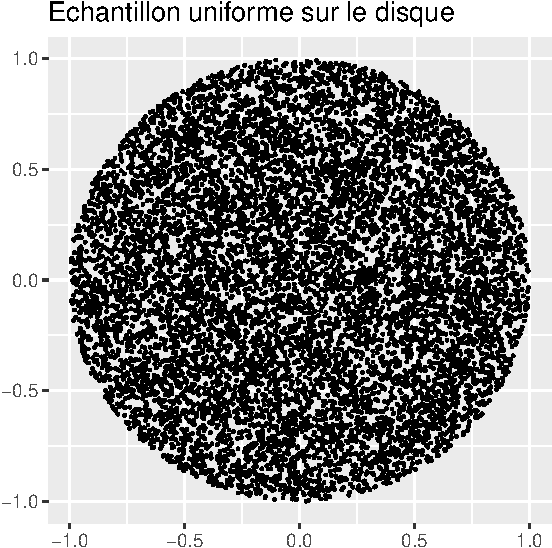
\includegraphics{correction_simulation_variables_aleatoires_files/figure-latex/plot_disque-1} \end{center}

\begin{Correction}
On peut regarder la distribution empirique du nombre d'essais moyens.
La théorie stipule qu'il s'agit d'une loi géométrique sur $\mathbb{N}^*$ de paramètre $\frac{\pi}{4}$.
\end{Correction}

\begin{Shaded}
\begin{Highlighting}[]
\NormalTok{k_max <-}\StringTok{ }\KeywordTok{max}\NormalTok{(disc_sample}\OperatorTok{$}\NormalTok{n_essai)}
\CommentTok{# D'abord en calcule les fréquences empiriques puis théoriques}
\NormalTok{disc_sample }\OperatorTok\StringTok{ }
\StringTok{  }\KeywordTok{mutate}\NormalTok{(}\DataTypeTok{n_essai =} \KeywordTok{factor}\NormalTok{(n_essai, }\DataTypeTok{levels =} \DecValTok{1}\OperatorTok{:}\NormalTok{k_max)) }\OperatorTok\StringTok{ }\CommentTok{# On transforme en facteur}
\StringTok{  }\KeywordTok{group_by}\NormalTok{(n_essai) }\OperatorTok\StringTok{ }\CommentTok{# Regroupement}
\StringTok{  }\KeywordTok{summarise}\NormalTok{(}\DataTypeTok{freq_empir =} \KeywordTok{n}\NormalTok{() }\OperatorTok{/}\StringTok{ }\NormalTok{n_sample) }\OperatorTok\StringTok{ }
\StringTok{  }\KeywordTok{ungroup}\NormalTok{() }\OperatorTok\StringTok{ }\CommentTok{# Degroupement}
\StringTok{  }\KeywordTok{mutate}\NormalTok{(}\DataTypeTok{freq_theo =} \KeywordTok{dgeom}\NormalTok{(}\DecValTok{0}\OperatorTok{:}\NormalTok{(k_max }\OperatorTok{-}\StringTok{ }\DecValTok{1}\NormalTok{), pi }\OperatorTok{/}\StringTok{ }\DecValTok{4}\NormalTok{)) }\OperatorTok\StringTok{ }\CommentTok{# Dans R, la loi geometrique}
\StringTok{  }\CommentTok{# est sur N, donc on retranche 1.}
\StringTok{  }\CommentTok{# Puis on transforme légèrement pour le graphique}
\StringTok{  }\KeywordTok{gather}\NormalTok{(}\OperatorTok{-}\NormalTok{n_essai, }\DataTypeTok{key =} \StringTok{"Distribution"}\NormalTok{, }\DataTypeTok{value =} \StringTok{"Proba"}\NormalTok{) }\OperatorTok\StringTok{ }\CommentTok{# Regardez ce que ca fait!}
\StringTok{  }\KeywordTok{ggplot}\NormalTok{() }\OperatorTok{+}\StringTok{ }\CommentTok{# on représente le résultat}
\StringTok{  }\KeywordTok{aes}\NormalTok{(}\DataTypeTok{x =}\NormalTok{ n_essai, }\DataTypeTok{y =}\NormalTok{ Proba) }\OperatorTok{+}\StringTok{ }\CommentTok{# }
\StringTok{  }\KeywordTok{geom_col}\NormalTok{(}\DataTypeTok{mapping =} \KeywordTok{aes}\NormalTok{(}\DataTypeTok{fill =}\NormalTok{ Distribution), }\CommentTok{# Ordonnée des fréquences empiriques}
           \DataTypeTok{width =} \FloatTok{0.3}\NormalTok{, }\DataTypeTok{position =} \StringTok{"dodge"}\NormalTok{) }\OperatorTok{+}
\StringTok{  }\KeywordTok{labs}\NormalTok{(}\DataTypeTok{x =} \StringTok{"k"}\NormalTok{, }\DataTypeTok{y =} \StringTok{"Probabilité"}\NormalTok{) }\OperatorTok{+}
\StringTok{  }\KeywordTok{scale_fill_discrete}\NormalTok{(}\DataTypeTok{labels =} \KeywordTok{c}\NormalTok{(}\StringTok{"Empirique"}\NormalTok{, }\StringTok{"Théorique"}\NormalTok{))}
\end{Highlighting}
\end{Shaded}

\begin{center}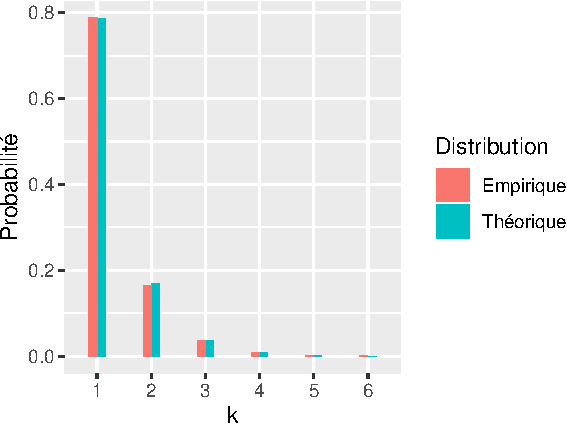
\includegraphics{correction_simulation_variables_aleatoires_files/figure-latex/nombre_essai-1} \end{center}

\hypertarget{proposition-optimale}{%
\subsection{Proposition optimale}\label{proposition-optimale}}

La loi normale tronquée de support \([b, +\infty[\) est définie par la
densité \(f\) proportionnelle, pour tout réel \(x\), à
\[f_1(x) = \exp\left\lbrace -\frac{(x-\mu)^2}{2\sigma^2}\right\rbrace\mathbf{1}_{x\geq b},
\quad\text{avec $\mu > 0$, $\sigma > 0$}.\]

On propose de simuler suivant la loi de densité \(f\) par une méthode de
rejet.

\hypertarget{muxe9thode-nauxefve}{%
\subsubsection{Méthode naïve}\label{muxe9thode-nauxefve}}

\begin{enumerate}
\def\labelenumi{\arabic{enumi}.}
\tightlist
\item
  On note \(\Phi\) la fonction de répartition de la loi normale centrée
  réduite. Montrer que \(f\) satisfait l'inégalité suivante pour tout
  réel \(x\):
  \[f(x)\leq \frac{1}{\sigma\sqrt{2\pi}\phi(\frac{\mu-b}{\sigma})}\exp\left\lbrace -\frac{(x-\mu)^2}{2\sigma^2}\right\rbrace.\]
\end{enumerate}

\begin{Correction}
On a que $f(x) \propto f_1(x)$. Donc
$$f(x) = \frac{f_1(x)}{\int_b^\infty f_1(z) \text{d} z}$$
Or:
\begin{align*}
\int_b^\infty f_1(z) \text{d} z &= \sqrt{2\pi\sigma^2} \int_{b}^\infty \frac{1}{\sqrt{2\pi\sigma^2}} \text{e}^{-\frac{(z - \mu)^2}{2 \sigma^2}}\\
&= \sqrt{2\pi\sigma^2} \mathbb{P}\left(\mu + \sigma Z > b\right)
\intertext{où $Z \sim \mathcal{N}(0,1)$}
& = \sqrt{2\pi\sigma^2} \mathbb{P}\left(Z > \frac{b - \mu}{\sigma} \right)\\
\\
& = \sqrt{2\pi\sigma^2} \mathbb{P}\left(Z < \frac{\mu - b}{\sigma}\right)
\end{align*}
Donc $$f(x)\leq \frac{1}{\sigma\sqrt{2\pi}\phi(\frac{\mu-b}{\sigma})}\exp\left\lbrace -\frac{(x-\mu)^2}{2\sigma^2}\right\rbrace\mathbf{1}_{x\geq b},$$
qui satisfait bien l'inéquation voulue.
\end{Correction}

\begin{enumerate}
\def\labelenumi{\arabic{enumi}.}
\setcounter{enumi}{1}
\tightlist
\item
  En déduire l'algorithme du rejet. Que peut-on dire du nombre d'essais
  moyen avant acceptation ?
\end{enumerate}

\begin{Correction}
Donc, si on fait un algorithme de rejet avec commme loi de proposition $g$ la densité d'une Gaussienne de moyenne $\mu$ et variance $\sigma^2$.
On a alors:
$$\frac{f(x)}{g(x)} \leq \frac{1}{\phi(\frac{\mu-b}{\sigma})}$$
La probabilité d'acceptation est donc exactement $\phi(\frac{\mu-b}{\sigma})$.
Ainsi, si

\begin{itemize}
\item $b < \mu$ alors, la probabilité d'acceptation est supérieure à 0.5.
\item Si $b >> \mu$, alors la probabilité d'acceptation est très petite!
\end{itemize}
\end{Correction}

\hypertarget{une-distribution-instrumentale-alternative}{%
\subsubsection{Une distribution instrumentale
alternative}\label{une-distribution-instrumentale-alternative}}

On suppose que \(b > \mu\). On considère la loi exponentielle translatée
de \(b\), \(\tau\mathcal{E}(\lambda, b)\), de densité
\[g_{\lambda}(x) = \lambda e^{-\lambda(x-b)}\mathbf{1}_{x\geq b},\quad x\in\mathbb{R}.\]
3. Montrer pour \(x\geq b\) que
\[\frac{f_1(x)}{g_{\lambda}(x)}\leq \left\lbrace
\begin{array}{lr}
\frac{1}{\lambda}\exp\left\lbrace
    \lambda(\mu-b)+\frac{(\lambda\sigma)^2}{2}
    \right\rbrace & \text{si } \mu+\lambda\sigma^2 > b,\\
    \frac{1}{\lambda}\exp\left\lbrace
    -\frac{(b-\mu)^2}{2\sigma^2}
    \right\rbrace & \text{sinon}.
\end{array}
\right. \]

\begin{Correction}
Soit $x \geq b$:
\begin{align*}
\frac{f_1(x)}{g(x)} &= \frac{1}{\lambda}\text{e}^{-\frac{(x - \mu)^2}{2\sigma^2} + \lambda(x - b)}\\
&= \frac{1}{\lambda}\text{e}^{-\frac{1}{2\sigma^2}\overbrace{\left((x - \mu)^2-2\sigma^2\lambda(x - b)\right)}^{:=P(x)}}
\intertext{où}
P(x) &= x^2 - 2\mu x - 2\lambda\sigma^2 x+ \mu^2 + 2\lambda\sigma^2 b\\
&= \left(x - (\mu + \lambda\sigma^2) \right)^2 - (\mu + \lambda\sigma^2)^2 + \mu^2 + 2\lambda\sigma^2 b\\
&=  \left(x - (\mu + \lambda\sigma^2) \right)^2 -2\sigma^2\left(\lambda(\mu - b) + \frac{\lambda^2\sigma^2}{2}  \right).
% \intertext{Donc:}
%\frac{f_1(x)}{g(x)} &= \frac{1}{\lambda}\text{e}^{-\frac{\left(x - (\mu + \lambda\sigma^2) \right)^2}{2\sigma^2} + \lambda(\mu - b) + \frac{\lambda^2\sigma^2}{2} }
\end{align*}
On travaille sur l'ensembke $x\geq b$. Ainsi, si $\mu + \lambda\sigma^2 > b$ $P(x)$ atteint son minimum en $x = \mu + \lambda\sigma^2.$ et le maximum du ratio est atteint en cette valeur.
Si $\mu + \lambda\sigma^2 \leq b$, $P(x)$ est minimal (donc le ratio maximal), en $x = b$.
On retrouve donc l'expression cherchée.
\end{Correction}

\begin{enumerate}
\def\labelenumi{\arabic{enumi}.}
\setcounter{enumi}{3}
\tightlist
\item
  Proposer une méthode de simulation de la loi de densité \(f\).
\end{enumerate}

\begin{Correction}
Ainsi à $b, \mu, et \sigma^2$ fixés, il suffit, pour un $\lambda$ choisi,

\begin{enumerate}
\item De calculer $M(\lambda)$ comme une des deux valeurs données plus haut, selon
que $\mu + \lambda\sigma^2 > b$ ou non.
\item De simuler $Y$ comme une exponentielle de paramètre $\lambda$, à laquelle on ajoute
$b$.
\item Simuler une uniforme $U\sim \mathcal{U}[0, 1]$;
\item Si $U < \frac{f_1(Y)}{M(\lambda)g(Y)}$, alors on pose $X = Y$, sinon, on recommence.
\end{enumerate}
\end{Correction}

\begin{enumerate}
\def\labelenumi{\arabic{enumi}.}
\setcounter{enumi}{4}
\tightlist
\item
  Calculer la valeur de \(\lambda^*\) telle que le temps moyen de calcul
  de la méthode proposée soit le plus petit possible.
\end{enumerate}

\begin{Correction}
On veut minimiser:

$$M(\lambda) = \left\lbrace
\begin{array}{lr}
\frac{1}{\lambda}\exp\left\lbrace
    \lambda(\mu-b)+\frac{(\lambda\sigma)^2}{2}
    \right\rbrace & \text{si } \lambda > \frac{b - \mu}{\sigma^2},\\
    \frac{1}{\lambda}\exp\left\lbrace
    -\frac{(b-\mu)^2}{2\sigma^2}
    \right\rbrace & \text{si } 0< \lambda \leq \frac{b - \mu}{\sigma^2}.
\end{array}
\right. $$

Sur l'intervalle $]0, \frac{b - \mu}{\sigma^2}]$, $M(\lambda)$ est décroissante,
le minimum est donc atteint $\frac{b - \mu}{\sigma^2}$. On notera que
$M(\lambda)$ est continue en ce point, et donc continue partout.

Sur $]\frac{b - \mu}{\sigma^2}, +\infty[$, on a
$$M'(\lambda) = \frac{1}{\lambda}M(\lambda)\left(\sigma^2 \lambda^2 + \lambda(\mu -b) - 1\right)$$

Ainsi, la dérivée est négative entre les deux solutions du polynôme qui sont:

$$\lambda_1 = \frac{(b - \mu) - \sqrt{(b-\mu)^2 + 4\sigma^2}}{2 \sigma^2} < 0$$

$$\lambda_2 = \frac{(b - \mu) + \sqrt{(b-\mu)^2 + 4\sigma^2}}{2 \sigma^2} > \frac{b - \mu}{\sigma^2}$$

Ainsi, le minimum global de $M(\lambda)$ est atteint en $\lambda_2$.
On a donc $\lambda^* = \lambda_2$.
\end{Correction}

\begin{enumerate}
\def\labelenumi{\arabic{enumi}.}
\setcounter{enumi}{5}
\tightlist
\item
  En \texttt{R}, mettre en oeuvre cette dernière méthode.
\end{enumerate}

\begin{Shaded}
\begin{Highlighting}[]
\CommentTok{# On définit les fonctions apparaissant}
\NormalTok{f1 <-}\StringTok{ }\ControlFlowTok{function}\NormalTok{(xs, b, mu, sigma2)\{}
  \KeywordTok{ifelse}\NormalTok{(}\DataTypeTok{test =}\NormalTok{ xs }\OperatorTok{>=}\StringTok{ }\NormalTok{b,}
         \DataTypeTok{yes =} \KeywordTok{exp}\NormalTok{(}\OperatorTok{-}\FloatTok{0.5} \OperatorTok{*}\StringTok{ }\NormalTok{(xs }\OperatorTok{-}\StringTok{ }\NormalTok{mu)}\OperatorTok{^}\DecValTok{2} \OperatorTok{/}\StringTok{ }\NormalTok{sigma2),}
         \DataTypeTok{no =} \DecValTok{0}\NormalTok{)}
\NormalTok{\}}

\NormalTok{target_f <-}\StringTok{ }\ControlFlowTok{function}\NormalTok{(xs, b, mu, sigma2)\{}
\NormalTok{  constante_normalisation <-}\StringTok{ }\KeywordTok{sqrt}\NormalTok{(}\DecValTok{2} \OperatorTok{*}\StringTok{ }\NormalTok{pi }\OperatorTok{*}\StringTok{ }\NormalTok{sigma2) }\OperatorTok{*}\StringTok{ }\KeywordTok{pnorm}\NormalTok{((mu }\OperatorTok{-}\StringTok{ }\NormalTok{b) }\OperatorTok{/}\StringTok{ }\NormalTok{sigma2)}
  \KeywordTok{f1}\NormalTok{(xs, b, mu, sigma2) }\OperatorTok{/}\StringTok{ }\NormalTok{constante_normalisation}
\NormalTok{\}}

\NormalTok{g_lambda <-}\StringTok{ }\ControlFlowTok{function}\NormalTok{(xs, b, lambda)\{}
  \KeywordTok{ifelse}\NormalTok{(xs }\OperatorTok{>}\StringTok{ }\NormalTok{b, lambda }\OperatorTok{*}\StringTok{ }\KeywordTok{exp}\NormalTok{(}\OperatorTok{-}\NormalTok{lambda }\OperatorTok{*}\StringTok{ }\NormalTok{(xs }\OperatorTok{-}\StringTok{ }\NormalTok{b)), }\DecValTok{0}\NormalTok{)}
\NormalTok{\}}

\NormalTok{get_lambda_opt <-}\StringTok{ }\ControlFlowTok{function}\NormalTok{(b, mu, sigma2)\{}
  \FloatTok{0.5} \OperatorTok{*}\StringTok{ }\NormalTok{(b }\OperatorTok{-}\StringTok{ }\NormalTok{mu }\OperatorTok{+}\StringTok{ }\KeywordTok{sqrt}\NormalTok{((b }\OperatorTok{-}\StringTok{ }\NormalTok{mu)}\OperatorTok{^}\DecValTok{2} \OperatorTok{+}\StringTok{ }\DecValTok{4} \OperatorTok{*}\StringTok{ }\NormalTok{sigma2)) }\OperatorTok{/}\StringTok{ }\NormalTok{sigma2}
\NormalTok{\}}

\NormalTok{get_M_lambda <-}\StringTok{ }\ControlFlowTok{function}\NormalTok{(lambdas, b, mu, sigma2)\{}
  \KeywordTok{ifelse}\NormalTok{(lambdas }\OperatorTok{>}\StringTok{ }\NormalTok{((b }\OperatorTok{-}\StringTok{ }\NormalTok{mu) }\OperatorTok{/}\StringTok{ }\NormalTok{sigma2),}
         \DataTypeTok{yes =} \KeywordTok{exp}\NormalTok{(lambdas }\OperatorTok{*}\StringTok{ }\NormalTok{(mu }\OperatorTok{-}\StringTok{ }\NormalTok{b) }\OperatorTok{+}\StringTok{ }\FloatTok{0.5} \OperatorTok{*}\StringTok{ }\NormalTok{sigma2 }\OperatorTok{*}\StringTok{ }\NormalTok{lambdas}\OperatorTok{^}\DecValTok{2}\NormalTok{ ) }\OperatorTok{/}\StringTok{ }\NormalTok{lambdas,}
         \DataTypeTok{no =} \KeywordTok{exp}\NormalTok{(}\OperatorTok{-}\FloatTok{0.5} \OperatorTok{*}\StringTok{ }\NormalTok{(b }\OperatorTok{-}\StringTok{ }\NormalTok{mu)}\OperatorTok{^}\DecValTok{2} \OperatorTok{/}\StringTok{ }\NormalTok{sigma2) }\OperatorTok{/}\StringTok{ }\NormalTok{lambdas)}
\NormalTok{\}}
\end{Highlighting}
\end{Shaded}

\begin{Correction}
Avec ces fonctions, on peut définir l'algorithme de simulation
\end{Correction}

\begin{Shaded}
\begin{Highlighting}[]
\NormalTok{mon_random_f <-}\StringTok{ }\ControlFlowTok{function}\NormalTok{(n, b, mu, sigma2)\{}
\NormalTok{  lambda_opt <-}\StringTok{ }\KeywordTok{get_lambda_opt}\NormalTok{(b, mu, sigma2)}\CommentTok{# On calcule le lambda optimal}
\NormalTok{  M <-}\StringTok{ }\KeywordTok{get_M_lambda}\NormalTok{(lambda_opt, b, mu, sigma2)}\CommentTok{# Le M de l'acceptation rejet}
\NormalTok{  get_one_sample <-}\StringTok{ }\ControlFlowTok{function}\NormalTok{()\{}
\NormalTok{    n_essai <-}\StringTok{ }\DecValTok{0}
\NormalTok{    accepted <-}\StringTok{ }\OtherTok{FALSE}
    \ControlFlowTok{while}\NormalTok{(}\OperatorTok{!}\NormalTok{accepted)\{}
\NormalTok{      n_essai =}\StringTok{ }\NormalTok{n_essai }\OperatorTok{+}\StringTok{ }\DecValTok{1}
\NormalTok{      candidat <-}\StringTok{ }\NormalTok{b }\OperatorTok{+}\StringTok{ }\KeywordTok{rexp}\NormalTok{(}\DecValTok{1}\NormalTok{, lambda_opt) }\CommentTok{# Exponentielle translatee}
\NormalTok{      ratio <-}\StringTok{ }\KeywordTok{f1}\NormalTok{(candidat, b, mu, sigma2) }\OperatorTok{/}\StringTok{ }\NormalTok{(M }\OperatorTok{*}\StringTok{ }\KeywordTok{g_lambda}\NormalTok{(candidat, b, lambda_opt))}
\NormalTok{      u <-}\StringTok{ }\KeywordTok{runif}\NormalTok{(}\DecValTok{1}\NormalTok{)}
\NormalTok{      accepted <-}\StringTok{ }\NormalTok{(u }\OperatorTok{<=}\StringTok{ }\NormalTok{ratio)}
\NormalTok{    \}}
    \KeywordTok{tibble}\NormalTok{(}\DataTypeTok{x =}\NormalTok{ candidat, }\DataTypeTok{n_essai =}\NormalTok{ n_essai)}
\NormalTok{  \}}
  \CommentTok{# On répète n_fois la même fonction, qui renvoie un tibble}
  \CommentTok{# tous les résultats sont ensuite concaténés}
\NormalTok{  res <-}\StringTok{ }\NormalTok{purrr}\OperatorTok{::}\KeywordTok{rerun}\NormalTok{(n, }\KeywordTok{get_one_sample}\NormalTok{()) }\OperatorTok\CommentTok{#}
\StringTok{    }\NormalTok{dplyr}\OperatorTok{::}\KeywordTok{bind_rows}\NormalTok{() }\CommentTok{# Concatenation}
  \KeywordTok{return}\NormalTok{(res)}
\NormalTok{\}}
\end{Highlighting}
\end{Shaded}

\begin{Correction}
Que l'on fait tourner pour certaines valeurs de $b$, $\mu$ et $\sigma^2$
\end{Correction}

\begin{Shaded}
\begin{Highlighting}[]
\NormalTok{b <-}\StringTok{ }\DecValTok{10}\NormalTok{; mu <-}\StringTok{ }\DecValTok{5}\NormalTok{; sigma2 <-}\StringTok{ }\DecValTok{1} \CommentTok{# paramètres}
\NormalTok{trunc_normal_samples <-}\StringTok{ }\KeywordTok{mon_random_f}\NormalTok{(}\DecValTok{10000}\NormalTok{, b, mu, sigma2)}
\end{Highlighting}
\end{Shaded}

\begin{Shaded}
\begin{Highlighting}[]
\NormalTok{my_breaks <-}\StringTok{ }\KeywordTok{c}\NormalTok{(}\DecValTok{0}\NormalTok{, }\KeywordTok{seq}\NormalTok{(b, b }\OperatorTok{+}\StringTok{ }\NormalTok{mu, }\DataTypeTok{length.out =} \DecValTok{51}\NormalTok{))}
\KeywordTok{ggplot}\NormalTok{(trunc_normal_samples, }\KeywordTok{aes}\NormalTok{(}\DataTypeTok{x =}\NormalTok{ x)) }\OperatorTok{+}
\StringTok{  }\KeywordTok{geom_histogram}\NormalTok{(}\KeywordTok{aes}\NormalTok{(}\DataTypeTok{y =}\NormalTok{ ..density..), }\DataTypeTok{breaks =}\NormalTok{ my_breaks,}
                 \DataTypeTok{fill =} \StringTok{"lightblue"}\NormalTok{) }\OperatorTok{+}
\StringTok{  }\KeywordTok{stat_function}\NormalTok{(}\DataTypeTok{fun =} \ControlFlowTok{function}\NormalTok{(x) }\KeywordTok{target_f}\NormalTok{(x, b, mu, sigma2), }\DataTypeTok{color =} \StringTok{"red"}\NormalTok{) }\OperatorTok{+}
\StringTok{  }\KeywordTok{labs}\NormalTok{(}\DataTypeTok{y =} \StringTok{"Densité"}\NormalTok{)}
\end{Highlighting}
\end{Shaded}

\begin{center}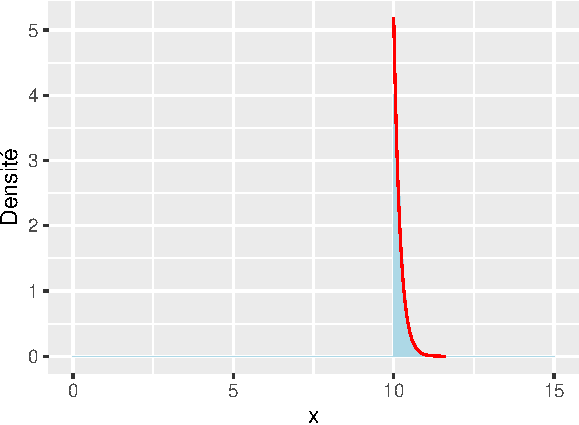
\includegraphics{correction_simulation_variables_aleatoires_files/figure-latex/representation_graphique-1} \end{center}

On verra dans l'exercice de la section 5 que la probabilité
d'acceptation peut être calculée ici. On peut aussi calculer la proba de
l'algo naif.

\begin{Shaded}
\begin{Highlighting}[]
\NormalTok{(proba_naive <-}\StringTok{ }\KeywordTok{pnorm}\NormalTok{((mu }\OperatorTok{-}\StringTok{ }\NormalTok{b) }\OperatorTok{/}\StringTok{ }\NormalTok{sigma2))}\CommentTok{# Proba de l'algo naif}
\end{Highlighting}
\end{Shaded}

\begin{verbatim}
[1] 2.866516e-07
\end{verbatim}

\begin{Shaded}
\begin{Highlighting}[]
\DecValTok{1} \OperatorTok{/}\StringTok{ }\KeywordTok{mean}\NormalTok{(trunc_normal_samples}\OperatorTok{$}\NormalTok{n_essai)}\CommentTok{# Proba empirique de l'algo optimisé}
\end{Highlighting}
\end{Shaded}

\begin{verbatim}
[1] 0.9821253
\end{verbatim}

\begin{Shaded}
\begin{Highlighting}[]
\CommentTok{# On peut en fait connaitre aussi la proba theorique (exo suivant)}
\NormalTok{lambda_star <-}\StringTok{ }\KeywordTok{get_lambda_opt}\NormalTok{(b, mu, sigma2)}
\NormalTok{M_star <-}\StringTok{ }\KeywordTok{get_M_lambda}\NormalTok{(lambda_star, b, mu, sigma2)}
\NormalTok{(proba_theo <-}\StringTok{ }\KeywordTok{sqrt}\NormalTok{(}\DecValTok{2} \OperatorTok{*}\StringTok{ }\NormalTok{pi }\OperatorTok{*}\StringTok{ }\NormalTok{sigma2) }\OperatorTok{*}\StringTok{ }\NormalTok{proba_naive }\OperatorTok{/}\StringTok{ }\NormalTok{M_star)}
\end{Highlighting}
\end{Shaded}

\begin{verbatim}
[1] 0.9827773
\end{verbatim}

\hypertarget{muxe9thode-de-transformation}{%
\section{Méthode de transformation}\label{muxe9thode-de-transformation}}

\hypertarget{simulation-de-lois-gaussiennes.-algorithme-de-box-muller}{%
\subsection{Simulation de lois Gaussiennes. Algorithme de
Box-Muller}\label{simulation-de-lois-gaussiennes.-algorithme-de-box-muller}}

Soient \(X\) et \(Y\) deux variables aléatoires indépendantes de loi
\(\mathcal{N}(0, 1)\)

\begin{enumerate}
\def\labelenumi{\arabic{enumi}.}
\tightlist
\item
  Montrer que si \(U\) et \(V\) sont deux variables aléatoires
  indépendantes de loi \(\mathcal{U}[0, 1]\) alors le couple
  \[\left(\sqrt{- 2 \ln(U)} \cos (2\pi V), \sqrt{- 2 \ln(U)} \sin(2\pi V)\right)\]
  a la même loi que le couple \((X, Y)\).
\end{enumerate}

\begin{Correction}
Pour $(u, v) \in ]0,1[^2$, on note 
$$\phi(u, v) = \left(\sqrt{- 2 \ln(u)} \cos (2\pi v), \sqrt{- 2 \ln(u)} \sin(2\pi v)\right)$$
On peut remarquer que pour tout $(x, y) \in \mathbb{R}^2_*$, la fonction définie par

$$\phi^{-1}(x, y) = 
\left\lbrace
\begin{array}{lr}
\left(\exp(-(x^2 + y^2)/2),  \frac{\arctan(y / x)}{2\pi} \right) & \text{ si } x > 0,~ y \geq 0\\
\left(\exp(-(x^2 + y^2)/2),  \frac{\arctan(y / x) + 2\pi}{2\pi} \right) & \text{ si } x > 0,~ y < 0\\
\left(\exp(-(x^2 + y^2)/2),  \frac{\arctan(y / x) + \pi}{2\pi} \right) & \text{ si } x < 0\\
\left(\exp(-(x^2 + y^2)/2),  \frac{1}{4} \right) & \text{ si } x = 0, y > 0\\
\left(\exp(-(x^2 + y^2)/2),  \frac{3}{4} \right) & \text{ si } x = 0, y < 0
\end{array}
\right.$$
est l'inverse de $\phi$. Ainsi, si tout les intervalles où $\phi^{-1}$
Ainsi, sur tout intervalle où cette fonction est différentiable, on peut écrire la Jacobienne
$$J_{\phi^{-1}}(x, y) = \begin{pmatrix}
\frac{\delta \phi^{-1}_1}{\delta x}(x, y) & \frac{\delta \phi^{-1}_1}{\delta y}(x, y)\\
\frac{\delta \phi^{-1}_2}{\delta x}(x, y) & \frac{\delta \phi^{-1}_2}{\delta y}(x, y)
\end{pmatrix}
=
\begin{pmatrix}
-x \text{e}^{-\frac{1}{2}(x ^2 + y^2)} &
-y \text{e}^{-\frac{1}{2}(x ^2 + y^2)} \\
\frac{1}{2\pi}\frac{-y}{x^2 + y ^2} &
\frac{1}{2\pi}\frac{x}{x^2 + y ^2}
\end{pmatrix}.$$

Ainsi, par formule du changement de variable, la densité $f_{X,Y}(x, y)$ du couple de variables aléatoires $(X, Y)$ est donnée par:

$$f_{X,Y}(x, y) = f_{U,V}(\phi^{-1}(x, y))\vert\det J_{\phi^{-1}}(x, y)\vert = \frac{1}{2\pi}\text{e}^{-\frac{1}{2}(x ^2 + y^2)} =  \frac{1}{\sqrt{2\pi}}\text{e}^{-\frac{1}{2}x^2}\frac{1}{\sqrt{2\pi}}\text{e}^{-\frac{1}{2}y^2}$$

On peut ainsi prolonger par continuité la fonction $f_{X, Y}$ en tous les points de discontinuité de $\phi^{-1}$.
Le couple $(X, Y)$ est donc un couple de 2 variables aléatoires indépendantes, de loi $\mathcal{N}(0, 1)$.
\end{Correction}

\begin{enumerate}
\def\labelenumi{\arabic{enumi}.}
\setcounter{enumi}{1}
\tightlist
\item
  Ecrire une fonction \texttt{box\_muller} permettant de simuler une loi
  \(\mathcal{N}(0, 1)\) en \texttt{R}. Vous comparerez l'histogramme
  obtenu à la vrai densité de la loi.
\end{enumerate}

\begin{Shaded}
\begin{Highlighting}[]
\NormalTok{box_muller <-}\StringTok{ }\ControlFlowTok{function}\NormalTok{(n_sample)\{}
\NormalTok{  n_uniform_sample <-}\StringTok{ }\KeywordTok{ceiling}\NormalTok{(}\FloatTok{0.5} \OperatorTok{*}\StringTok{ }\NormalTok{n_sample)}
\NormalTok{  u <-}\StringTok{ }\KeywordTok{runif}\NormalTok{(n_uniform_sample)}
\NormalTok{  v <-}\StringTok{ }\KeywordTok{runif}\NormalTok{(n_uniform_sample)}
\NormalTok{  first_half <-}\StringTok{ }\KeywordTok{sqrt}\NormalTok{(}\OperatorTok{-}\DecValTok{2} \OperatorTok{*}\StringTok{ }\KeywordTok{log}\NormalTok{(u)) }\OperatorTok{*}\StringTok{ }\KeywordTok{cos}\NormalTok{(}\DecValTok{2} \OperatorTok{*}\StringTok{ }\NormalTok{pi }\OperatorTok{*}\StringTok{ }\NormalTok{v)}
\NormalTok{  second_half <-}\StringTok{ }\KeywordTok{sqrt}\NormalTok{(}\OperatorTok{-}\DecValTok{2} \OperatorTok{*}\StringTok{ }\KeywordTok{log}\NormalTok{(u)) }\OperatorTok{*}\StringTok{ }\KeywordTok{sin}\NormalTok{(}\DecValTok{2} \OperatorTok{*}\StringTok{ }\NormalTok{pi }\OperatorTok{*}\StringTok{ }\NormalTok{v)}
  \KeywordTok{tibble}\NormalTok{(}\DataTypeTok{sample =} \KeywordTok{c}\NormalTok{(first_half, second_half))}
\NormalTok{\}}
\end{Highlighting}
\end{Shaded}

\begin{Shaded}
\begin{Highlighting}[]
\KeywordTok{box_muller}\NormalTok{(}\FloatTok{1e4}\NormalTok{) }\OperatorTok\StringTok{ }
\StringTok{  }\KeywordTok{ggplot}\NormalTok{(}\KeywordTok{aes}\NormalTok{(}\DataTypeTok{x =}\NormalTok{ sample)) }\OperatorTok{+}
\StringTok{  }\KeywordTok{geom_histogram}\NormalTok{(}\KeywordTok{aes}\NormalTok{(}\DataTypeTok{y =}\NormalTok{ ..density..), }\DataTypeTok{fill =} \StringTok{"lightblue"}\NormalTok{) }\OperatorTok{+}
\StringTok{  }\KeywordTok{stat_function}\NormalTok{(}\DataTypeTok{fun =}\NormalTok{ dnorm) }\OperatorTok{+}
\StringTok{  }\KeywordTok{labs}\NormalTok{(}\DataTypeTok{x =} \StringTok{"Valeur"}\NormalTok{, }\DataTypeTok{y =} \StringTok{"Densité"}\NormalTok{)}
\end{Highlighting}
\end{Shaded}

\begin{center}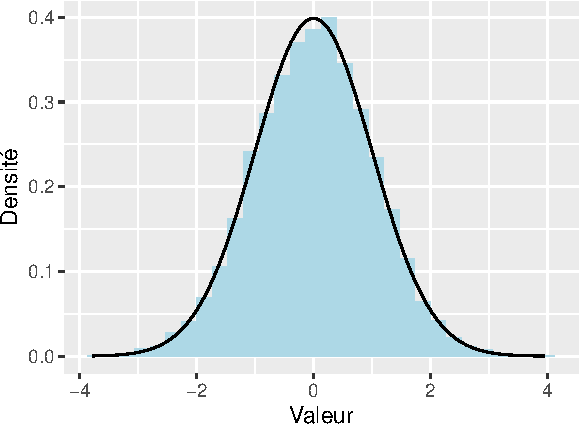
\includegraphics{correction_simulation_variables_aleatoires_files/figure-latex/plot_box_muller-1} \end{center}

\begin{enumerate}
\def\labelenumi{\arabic{enumi}.}
\setcounter{enumi}{2}
\tightlist
\item
  En déduire, pour tout \(\mu \in \mathbb{R^2}\) et toute matrice
  \(2\times 2\) symmétrique semi-définie positive \(\Sigma\) une méthode
  pour simuler une variable aléatoire
  \(Z\sim \mathcal{N}(\mu, \Sigma)\).
\end{enumerate}

\begin{Correction}
Pour toute matrice semi définie positive $\Sigma$, on peut définir une unique matrice triangulaire inférieure, notée $\Sigma^{\frac{1}{2}}$, telle que $\Sigma^{\frac{1}{2}}(\Sigma^{\frac{1}{2}})^T = \Sigma$ (cette matrice est la transposée de la décomposition de Choleski).
De plus, on rappelle que si $X \sim \mathcal{N}(0, I)$, alors, pour un vecteur a et une matrice B de dimensions adéquates $\mu + BX \sim \mathcal{N}(\mu, BB^T)$. À partir de l'algorithme de Box-Muller, on peut donc simuler n'importe quel vecteur Gaussien.
\end{Correction}

\hypertarget{autour-de-laccepation-rejet}{%
\section{Autour de l'accepation
rejet}\label{autour-de-laccepation-rejet}}

\hypertarget{acceptation-rejet-uxe9tendu-cas-de-deux-fonctions-positives.}{%
\subsection{Acceptation rejet étendu: Cas de deux fonctions
positives.}\label{acceptation-rejet-uxe9tendu-cas-de-deux-fonctions-positives.}}

\emph{Pour cette preuve, vous pourrez mimer les étapes de la preuve dans
le cas usuel, détaillée dans le poly.}

On se propose de montrer que pour que simuler selon une densité par
algorithme d'acceptation rejet, il n'est nécessaire de connaître la
densité qu'\emph{à la constante de normalisation près}. Cette propriété
est très utile dans le cas où le calcul de la constante de normalisation
est coûteux, voir impossible (typiquement en statistiques Bayesiennes).

Plus formellement, soient \(\tilde{f}\) une fonction positive et \(g\)
une densité de probabilité, toutes deux définies sur \(\mathbb{R}^d\)
telles que:

\begin{itemize}
\tightlist
\item
  \(0 < \int_{\mathbb{R}^d}\tilde{f}(x)\text{d}x < \infty\) . On note
  respectivement \(I(\tilde{f})\) cette intégrale et \begin{align*}
  f(x) &= \frac{\tilde{f}(x)}{I(\tilde{f})}
  \end{align*} la densité associée à cette fonction positive.
\item
  Il existe \(M>0\) tel que, pour tout réel \(x\),
  \(\tilde{f}(x) \leq M g(x)\).
\end{itemize}

On note \[\alpha(x) := \frac{\tilde{f}(x)}{Mg(x)}.\] Soit
\((U_m)_{m\geq 1}\) une suite de variables aléatoires i.i.d. de loi
uniforme sur \([0, 1]\). Soit \((Y_m)_{m\geq 1}\) une suite de variables
aléatoires indépendantes et identiquement distributée, de densité donnée
par \(g\). On note \(T\) la variable aléatoire (à valeurs dans
\(\mathbb{N}^*\)):
\[T = \inf\left\lbrace m, \text{ tel que } U_m \leq \alpha(Y_m)\right\rbrace.\].

\begin{enumerate}
\def\labelenumi{\arabic{enumi}.}
\tightlist
\item
  Montrer la variable aléatoire \(X := Y_T\) (\(T\)-ième valeur de la
  suite \((Y_m)_{m\geq 1}\)) a pour densité \(f\).
\end{enumerate}

\begin{Correction}
On reprend, à la normalisation près, la démonstration du cours:

Soit un entier $n\leq 1$:
\begin{align*}
\mathbb{P}\left(X\leq x, T = n \right) &=  \mathbb{P}\left( U_1 > \alpha(Y_1), \dots, U_{n - 1} > \alpha(Y_{n-1}), U_n \leq \alpha(Y_n), Y_n \leq x  \right)
\intertext{Par propriété d'indépendance}
&= \mathbb{P}\left(U_n \leq \alpha(Y_n), Y_n \leq x  \right)\prod_{i = 1}^{n-1}\mathbb{P}\left(U_i > \alpha(Y_i)\right)
\intertext{Par propriété de distribution identique}
&= \mathbb{P}\left(U_n \leq \alpha(Y_n), Y_n \leq x  \right)\mathbb{P}\left(U_1 > \alpha(Y_1)\right)^{n-1}
%%%%%% PREMIER TERME%%%%
\intertext{Or on a:}
\mathbb{P}\left(U_1 > \alpha(Y_1)\right) &= \mathbb{E}\left[\mathbf{1}_{U_1 > \alpha(Y_1)}\right]\\
&= \int_{\mathbb{R}} \left(\int_0^1 \mathbf{1}_{u > \frac{\tilde{f}(y)}{Mg(y)}} \text{d}  u\right)\times g(y) \text{d} y\\
&=\int_{\mathbb{R}} \left(1 -  \frac{I(\tilde{f})f(y)}{Mg(y)}\right)g(y) \text{d} y
\intertext{Comme $f$ est une densité:}
\mathbb{P}\left(U_1 > \alpha(Y_1)\right) &=1 - \frac{I(\tilde{f})}{M}
%%%%%% SECONDTERME%%%%
\intertext{De manière analogue}
\mathbb{P}\left(U_n \leq \alpha(Y_n), Y_n \leq x  \right) &= \mathbb{E}\left[\mathbf{1}_{U_n \leq \alpha(Y_n)}\times \mathbf{1}_{Y_n \leq x}\right]\\
&=  \int_{\mathbb{R}} \left(\int_0^1 \mathbf{1}_{u \leq \frac{f(y)}{Mg(y)}} \text{d}  u\right)\times \mathbf{1}_{y \leq x} g(y) \text{d} y\\
&= \int_{-\infty}^x \frac{I(\tilde{f})f(y)}{M}\text{d} y\\
&= \frac{I(\tilde{f})F(x)}{M},
\intertext{où $F(x)$ est la fonction de répartition associée à $f$. En résumé:}
\mathbb{P}\left(X\leq x, T = n \right) &= \frac{I(\tilde{f})F(x)}{M}\left(1 - \frac{I(\tilde{f})}{M}\right)^{n - 1}
\end{align*}
Donc on conclut en remarquant que  
$$\mathbb{P}(X\leq x) = \sum_{n = 1}^\infty \mathbb{P}\left(X\leq x, T = n \right) = F(x)$$
\end{Correction}

\begin{enumerate}
\def\labelenumi{\arabic{enumi}.}
\setcounter{enumi}{1}
\tightlist
\item
  Donnez alors la loi de la variable aléatoire \(T\). Quelle est
  l'espérance de \(T\)?
\end{enumerate}

\begin{Correction}
De la preuve, on peut déduire que 
$$\mathbb{P}\left(T = n \right) = \lim_{x \rightarrow \infty}\mathbb{P}\left(X\leq x, T = n \right) = \lim_{x \rightarrow \infty} \frac{I(\tilde{f})F(x)}{M}\left(1 - \frac{I(\tilde{f})}{M}\right)^{n - 1} =  \frac{I(\tilde{f})}{M}\left(1 - \frac{I(\tilde{f})}{M}\right)^{n - 1}$$
Donc, la loi de $T$ est une loi géométrique sur $\mathbb{N}_*$ de paramètre $\frac{I(\tilde{f})}{M}$. 
L'espérance de $T$ est donc donnée par $\frac{M}{I(\tilde{f})}$.
\end{Correction}

\begin{enumerate}
\def\labelenumi{\arabic{enumi}.}
\setcounter{enumi}{2}
\tightlist
\item
  En déduire un estimateur de \(I(\tilde{f})\) par méthode de Monte
  Carlo, obtenu uniquement à partir de l'algorithme d'acceptation rejet
  défini plus tôt.
\end{enumerate}

\begin{Correction}
Supposons qu'on simule un échantillon $X_1,\dots,X_n$ de variables aléatoires i.i.d.
de densité $f$ par l'algorithme d'acceptation rejet. Pour chaque $X_i (1\leq i\leq n)$, on note $T_i$ le temps d'arrêt correspondant.

Ainsi, l'estimateur 
$$\hat{\tau}_n = \frac{1}{n}\sum_{i = 1}^nT_i$$ 
est un estimateur sans biais de $\frac{M}{I(\tilde{f})}$. Donc, $M$  étant connu,
$$\hat{I}_n(\tilde{f}) = \frac{M}{\hat{\tau}_n}$$
est un estimateur consistant de $I(\tilde{f})$.
\end{Correction}

\begin{enumerate}
\def\labelenumi{\arabic{enumi}.}
\setcounter{enumi}{3}
\tightlist
\item
  Grâce au théorème central limite, donnez l'expression d'un intervalle
  de confiance asymptotique à 95\% pour \(I(\tilde{f})\), ne dépendant
  d'aucune quantité inconnue.
\end{enumerate}

\begin{Correction}
Le théorème central limite nous donne:

$$\sqrt{n}\left(\hat{\tau}_n - \frac{M}{I(\tilde{f})}\right) \overset{loi}{\longrightarrow} \mathcal{N}\left(0, \sigma^2\right)$$
où $\sigma^2 = \mathbb{V}\left[\hat{\tau}_n\right]$.
Par la $\Delta$- méthode, on a que
$$\sqrt{n}\left(\hat{I}_n(\tilde{f}) - I(\tilde{f})\right) \overset{loi}{\longrightarrow} \mathcal{N}\left(0, \tilde{\sigma}^2\right)$$
où $\tilde{\sigma} = \frac{M^2}{\hat{\tau}_n^4}\sigma^2$

Or un estimateur consistant de $\sigma^2$ est 
$$S^2 = \frac{1}{n}\sum_{i = 1}^n\left(T_i - \hat{\tau}_n \right)^2$$
Donc
$$\frac{1}{n}\frac{M^2}{\hat{\tau}_n^4}S^2$$
est un estimateur consistant de la variance de $\hat{I}_n(\tilde{f})$.

Un intervalle de confiance asymptotique à 95\% est donc donné par:
$$\left[\hat{I}_n - 1.96 \frac{M}{\hat{\tau}_n^2}\sqrt{\frac{S^2}{n}};
\hat{I}_n + 1.96 \frac{M}{\hat{\tau}_n^2}\sqrt{\frac{S^2}{n}}\right]$$
\end{Correction}

\hypertarget{recyclage-dans-lacceptation-rejet}{%
\subsection{Recyclage dans l'acceptation
rejet}\label{recyclage-dans-lacceptation-rejet}}

\emph{Dans cette section, on se replace dans le cadre classique de
l'acceptation rejet}.

On se propose d'approcher une intégrale du type:
\(J = \mathbb{E}_f[\varphi(X)]\) où \(f(\) est la densité de la variable
aléatoire \(X\) sur \(\mathbb{R}^d\) selon laquelle on ne sait pas
simuler, et \(\varphi\) est une fonction intégrable par rapport à cette
densité.

À partir d'une densité \(g(x)\) sur \(\mathbb{R}^d\) selon laquelle on
sait simuler, et telle que
\[\exists M>0,\text{ tel que } \forall x\in \mathbb{R}^d,~f(x) \leq Mg(x)\]
on obtient, par algorithme d'acceptation-rejet (pour un tel \(M\) fixé)
un échantillon de variables aléatoires \(i.i.d.\) \(X_1,\dots, X_n\) de
loi donnée par \(f\).

Pour obtenir cet échantillon de taille \(n\), on a simulé \(N\geq n\)
variables aléatoires indépendantes \(Y_1,\dots, Y_N\) de densité \(g\).
On note \(Z_1,\dots,Z_{N - n}\) l'échantillon i.i.d. de variables
aléatoires ayant été rejetées dans l'algorithme d'acceptation rejet.

\begin{enumerate}
\def\labelenumi{\arabic{enumi}.}
\setcounter{enumi}{4}
\tightlist
\item
  Donner l'expression de la densité de la variable aléatoire \(Z_1\).
\end{enumerate}

\begin{Correction}
\begin{align*}
\mathbb{P}(Z_1 \leq z) &= \mathbb{P}\left(Y_1\leq z \vert U > \alpha(Y_1)\right)\\
&= \frac{\mathbb{P}\left(Y_1\leq z , U > \alpha(Y_1)\right)}{\mathbb{P}\left(U > \alpha(Y_1)\right)}
\end{align*}
Le dénominateur est égal à $1 - \frac{1}{M}$ (voir section précédente, ou le cours).
Intéressons nous au numérateur
\begin{align*}
\mathbb{P}\left(Y_1\leq z , U > \alpha(Y_1)\right) &= \mathbb{E}\left[\mathbf{1}_{Y_1\leq z} \mathbf{1}_{U > \alpha(Y_1)}\right]\\
&=\int_{\mathbb{R}}\int_{0}^{1} \mathbf{1}_{u > \alpha(y)} \text{d} u \mathbf{1}_{y \leq z} g(y) \text{d} y\\
&=\int_{\mathbb{R}} \left(1 - \frac{f(y)}{Mg(y)}\right)  \mathbf{1}_{y \leq z} g(y) \text{d} y\\
&= \int_{-\infty}^z g(y) - \frac{f(y)}{M} dy
\end{align*}
Ainsi, on a
$$\mathbb{P}(Z_1\leq z) = \frac{M}{M - 1} \int_{-\infty}^z g(y) - \frac{f(y)}{M} dy = \int_{-\infty}^z \frac{Mg(y) - f(y)}{M - 1} \text{d}y$$

La densité de $Z_1$ est donc $h(z) = \frac{Mg(z) - f(z)}{M - 1}$ 
\end{Correction}

\begin{enumerate}
\def\labelenumi{\arabic{enumi}.}
\setcounter{enumi}{5}
\tightlist
\item
  En déduire que
  \[\hat{J}_n = \frac{1}{N} \left(\sum_{i = 1}^n \varphi(X_i) + \sum_{j = 1}^{N - n} \frac{(M - 1)f(Z_j)}{Mg(Z_j) - f(Z_j)} \varphi(Z_j) \right)\]
  est un estimateur sans biais de \(J\). Quelle est l'intérêt de cette
  méthode selon vous?
\end{enumerate}

\begin{Correction}

On s'intéresse $\mathbb{E}[\hat{J}_N]$. Il faut ici remarquer que $N$ est également aléatoire. 
On passera par l'espérance conditionnelle
$$\mathbb{E}\left[\hat{J}_n\right] = \mathbb{E}\left[\mathbb{E}\left[\hat{J}_n\vert N\right] \right] = \mathbb{E}\left[ \frac{1}{N} \left(\sum_{i = 1}^n \mathbb{E}[\varphi(X_i)\vert N] + \sum_{j = 1}^{N - n} \mathbb{E}\left[\frac{(M - 1)f(Z_j)}{Mg(Z_j) - f(Z_j)} \varphi(Z_j)\right \vert N] \right) \right]$$

Chacune des espérances conditionnelles est égale $J$ (le premier, car c'est un estimateur Monte Carlo standard, le deuxième car c'est un estimateur par échantillonage préférentiel quand la loi de proposition est $h$!). Ainsi, $\hat{J}_n$ est bien d'espérance $J$. 

Cette méthode permet donc d'avoir un estimateur sans biais de $J$ à partir de tous les échantillons simulés pour l'acceptation rejet.
\end{Correction}

\hypertarget{application}{%
\subsection{Application}\label{application}}

On reprend l'exemple vu en cours d'introduction à la statistique
bayésienne. Vous reprendrez le même modèle ainsi que les mêmes données
utilisées.

\begin{enumerate}
\def\labelenumi{\arabic{enumi}.}
\setcounter{enumi}{6}
\tightlist
\item
  En utilisant le même prior que celui du cours, ainsi que le même loi
  de proposition \(g\), implémentez l'algorithme d'acceptation rejet
  pour tirer selon le posterior. Les algorithmes efficaces seront
  valorisés.
\end{enumerate}

\begin{Correction}
\textit{On reprend les notations du cours (voir poly ou diapos)}

Pour un échantillon observé $y_{1:n} = y_1,\dots, y_n$ et les covariables associées $\mathbf{x}_1,\dots,\mathbf{x}_n$, on pose un modèle probit. 
La vraisemblance est données par
$$L(y_{1:n}\vert \theta,\mathbf{x}_{1:n}) = \prod_{k = 1}^n \underset{\text{Proba. présence}}{\phi(\mathbf{x}_k^T\theta)^{y_k}}\times \underset{\text{Proba. absence}}{(1 - \phi(\mathbf{x}_k^T\theta))}^{1 - y_k}$$
où $\phi$ est la fonction de répartition d'une loi $\mathcal{N}(0, 1)$.

Sur les paramètres inconnus, on pose un prior $\pi(\theta)\sim \mathcal{N}(0, 4 I_4)$.
Le posterior est donc donné par:
$$\pi(\theta \vert y_{1:n}, \mathbf{x}_{1:n}) \propto \pi(\theta) L(y_{1:n}\vert \theta, \mathbf{x}_{1:n}) \propto \frac{1}{64\pi^2}\text{e}^{-\frac{1}{8}\theta^T\theta} \prod_{k = 1}^n \phi(\mathbf{x}_k^T\theta)^{y_k} (1 - \phi(\mathbf{x}_k^T\theta))^{1 - y_k}$$

On note 
$$\tilde{\pi}(\theta \vert y_{1:n}, \mathbf{x}_{1:n})) = \frac{1}{64\pi^2}\text{e}^{-\frac{1}{8}\theta^T\theta} \prod_{k = 1}^n \phi(\mathbf{x}_k^T\theta)^{y_k} (1 - \phi(\mathbf{x}_k^T\theta))^{1 - y_k}$$
Afin de simuler cette loi par acceptation rejet, on choisit comme loi de proposition la loi du prior (i.e. $g(\theta) = \pi(\theta)$).
On remarque ainsi que pour tout $\theta$,
$$\frac{\tilde{\pi}(\theta \vert y_{1:n}, \mathbf{x}_{1:n}))}{g(\theta)} =  L(y_{1:n}\vert \theta, \mathbf{x}_{1:n})$$

De par l'expression de la vraisemblance, un majorant naturel, noté $\tilde{M}$ de ce ratio est 1.

Cependant, un majorant plus efficace est donné par la valeur du maximum de vraisemblance. Cette valeur est celle calculée pour effectuer l'inférence "classique".

Ainsi, en trouvant cette valeur, on obtiendra un $\tilde{M}$ qui sera plus petit, donc la probabilité d'acceptation (donnée en question 2.) sera plus grande.

Notre algorithme pour obtenir un échantillon du posterior est donc le suivant:

\begin{enumerate}
\item Trouver $\tilde{M} = \max_\theta L(y_{1:n}\vert \theta, \mathbf{x}_{1:n})$
\item Simuler un candidat $\theta_{cand} \sim \mathcal{N}(0, 4 I_4)$
\item Simuler (indépendemment de $U$) $U\sim\mathcal{U}[0,1]$.
\item Si $U \leq  \frac{L(y_{1:n}\vert \theta_{cand}, \mathbf{x}_{1:n})}{\tilde{M}}$, on accepte $\theta_{cand}$, sinon, on retourne à l'étape 2.
\end{enumerate}
\end{Correction}

\begin{enumerate}
\def\labelenumi{\arabic{enumi}.}
\setcounter{enumi}{7}
\tightlist
\item
  Implémentez cette méthode, et tracez les densités empiriques des
  posteriors obtenus. Vous donnerez également une estimation de
  \(\mathbb{E}[\theta \vert y_{1:n}]\) ainsi que l'intervalle de
  confiance associé.
\end{enumerate}

\begin{Correction}
La première chose à faire est d'écrire la fonction de vraisemblance. 
Elle prendra en entrée un vecteur de $\beta$, une matrice $X$ qui est la matrice de 
design, un vecteur $y$ de 0 et de 1, et un argument $\log$ qui sera utile pour éviter 
les problèmes numériques.
\end{Correction}

\begin{Shaded}
\begin{Highlighting}[]
\NormalTok{get_likelihood <-}\StringTok{ }\ControlFlowTok{function}\NormalTok{(beta_vec, }
\NormalTok{                           X, }\CommentTok{# Design matrix }
\NormalTok{                           y, }\CommentTok{# presence absence vector (numeric with 0 or 1) }
                           \DataTypeTok{return_log =} \OtherTok{FALSE}\NormalTok{)\{ }\CommentTok{# Return the loglikelihood, default: No}
\NormalTok{  X_beta <-}\StringTok{ }\KeywordTok{as.numeric}\NormalTok{(X }\OperatorTok\StringTok{ }\NormalTok{beta_vec) }\CommentTok{# The as.numeric returns a vector}
\NormalTok{  log_phi <-}\StringTok{ }\KeywordTok{pnorm}\NormalTok{(X_beta, }\DataTypeTok{log.p =}\NormalTok{ T) }\CommentTok{# Evaluates the phi. Taking the log}
  \CommentTok{# is a usual trick to avoid numerical problems}
  \CommentTok{# Ifelse vectorise binary tests}
\NormalTok{  log_probability <-}\StringTok{ }\KeywordTok{ifelse}\NormalTok{(}\DataTypeTok{test =}\NormalTok{ (y }\OperatorTok{==}\StringTok{ }\DecValTok{1}\NormalTok{), }\CommentTok{# Test if presence}
                           \DataTypeTok{yes =}\NormalTok{ log_phi, }\CommentTok{# Then the proba is phi(y)}
                           \DataTypeTok{no =} \KeywordTok{log}\NormalTok{(}\DecValTok{1} \OperatorTok{-}\StringTok{ }\KeywordTok{exp}\NormalTok{(log_phi))) }\CommentTok{# Else 1 - phi}
  \CommentTok{# Then, return either the result or its exponential (depending on return_log)}
  \KeywordTok{ifelse}\NormalTok{(return_log,}
         \DataTypeTok{yes =} \KeywordTok{return}\NormalTok{(}\KeywordTok{sum}\NormalTok{(log_probability)),}
         \DataTypeTok{no =} \KeywordTok{return}\NormalTok{(}\KeywordTok{exp}\NormalTok{(}\KeywordTok{sum}\NormalTok{(log_probability))))}
\NormalTok{\}}
\end{Highlighting}
\end{Shaded}

\begin{Correction}
On définit ensuite proprement la matrice de design ainsi que le vecteur de presence absence à partir des données
\end{Correction}

\begin{Shaded}
\begin{Highlighting}[]
\KeywordTok{library}\NormalTok{(tidyverse)}
\CommentTok{# Loading data}
\NormalTok{donnees_presence <-}\StringTok{ }\KeywordTok{read.table}\NormalTok{(}\StringTok{"https://papayoun.github.io/courses/2020_monte_carlo/enonces_td/donnees_presence.txt"}\NormalTok{,  }
                               \DataTypeTok{sep =} \StringTok{";"}\NormalTok{, }\DataTypeTok{header =} \OtherTok{TRUE}\NormalTok{, }
                               \DataTypeTok{colClasses =} \KeywordTok{c}\NormalTok{(}\DataTypeTok{presence =} \StringTok{"factor"}\NormalTok{))}
\CommentTok{# Creating design matrix}
\NormalTok{design_matrix <-}\StringTok{ }\NormalTok{donnees_presence }\OperatorTok\StringTok{ }\CommentTok{# A partir des données}
\StringTok{  }\KeywordTok{select}\NormalTok{(}\OperatorTok{-}\NormalTok{presence) }\OperatorTok\StringTok{ }\CommentTok{# On vire la colonne des presence }
\StringTok{  }\KeywordTok{as.matrix}\NormalTok{() }\OperatorTok\StringTok{ }\CommentTok{# On transforme en matrice}
\StringTok{  }\KeywordTok{cbind}\NormalTok{(}\DataTypeTok{intercept =} \KeywordTok{rep}\NormalTok{(}\DecValTok{1}\NormalTok{, }\KeywordTok{nrow}\NormalTok{(.)), .) }\CommentTok{# On colle à gauche une colonne }
\CommentTok{# remplie de 1 pour l'intercept}
\NormalTok{y_vector <-}\StringTok{ }\NormalTok{donnees_presence }\OperatorTok\StringTok{ }
\StringTok{  }\KeywordTok{pull}\NormalTok{(presence) }\OperatorTok\StringTok{ }\CommentTok{# On extrait la colonne presence (de type factor)}
\StringTok{  }\KeywordTok{as.character}\NormalTok{() }\OperatorTok\StringTok{ }\CommentTok{# on transforme en string}
\StringTok{  }\KeywordTok{as.numeric}\NormalTok{() }\CommentTok{# on transforme en numérique}
\end{Highlighting}
\end{Shaded}

\begin{Correction}
\textbf{Détermination de $\tilde{M}$ par optimisation de la vraisemblance}

Optimiser la vraisemblance du modèle probit est un problème classique en statistiques. 
La plupart des logiciels le font dans des fonctions dédiées (la fonction \texttt{glm} dans R, par exemple).
Ici, on peut utiliser une fonction d'optimisation numérique donnée par R (la fonction \texttt{optim}) pour le faire à notre place, de manière efficace. 
Afin de savoir utiliser cette fonction, on se réfèrera à \texttt{help(optim)}.


\textit{Remarque: } Ce cours n'étant pas un cours d'optimisation numérique, il n'est pas nécessaire de coder sa fonction soit même, ce qui serait fastidieux.
\end{Correction}

\begin{Shaded}
\begin{Highlighting}[]
\CommentTok{# On optimise par un algo de Nelder-Mead}
\CommentTok{# La fonction optim trouve le minimum d'une fonction}
\CommentTok{# Donc on veut minimiser -log_vraisemblance}
\NormalTok{M_tilde <-}\StringTok{ }\KeywordTok{optim}\NormalTok{(}\DataTypeTok{par =} \KeywordTok{rep}\NormalTok{(}\DecValTok{0}\NormalTok{, }\DecValTok{4}\NormalTok{), }\CommentTok{# point de depart de l'algorithm}
                 \DataTypeTok{fn =} \ControlFlowTok{function}\NormalTok{(b)\{ }\CommentTok{# Fonction a minimiser, }
                   \CommentTok{# On met les bons parametres}
                   \OperatorTok{-}\KeywordTok{get_likelihood}\NormalTok{(}\DataTypeTok{beta_vec =}\NormalTok{ b, }\DataTypeTok{X =}\NormalTok{ design_matrix, }
                                   \DataTypeTok{y =}\NormalTok{ y_vector, }\DataTypeTok{return_log =} \OtherTok{TRUE}\NormalTok{)}
\NormalTok{                   \})  }\OperatorTok\StringTok{  }\CommentTok{# Renvoie une liste}
\StringTok{  }\NormalTok{\{.}\OperatorTok{$}\NormalTok{value }\OperatorTok{*}\StringTok{ }\NormalTok{(}\OperatorTok{-}\DecValTok{1}\NormalTok{)\} }\OperatorTok\StringTok{ }\CommentTok{# dont on extrait la valeur du minimum * -1}
\StringTok{  }\KeywordTok{exp}\NormalTok{() }\CommentTok{# on se débarasse du logarithme}
\end{Highlighting}
\end{Shaded}

\begin{Correction}
La valeur optimale est donc d'à peu près 0.015. On est ainsi 66 fois plus efficace (en terme d'acceptation) que la borne $\tilde{M} = 1$.

On peut ainsi coder l'algorithme d'acceptation rejet. Dans cette fonction, en prévision de la suite, on conservera tous les candidats rejetés.
\end{Correction}

\begin{Shaded}
\begin{Highlighting}[]
\NormalTok{get_sample_accept_reject <-}\StringTok{ }\ControlFlowTok{function}\NormalTok{(X, }
\NormalTok{                                     y,}
\NormalTok{                                     M_bound)\{}
\NormalTok{  stop_condition <-}\StringTok{ }\OtherTok{FALSE} \CommentTok{# Stopping condition}
\NormalTok{  output_matrix <-}\StringTok{ }\OtherTok{NULL} \CommentTok{# Output matrix, will contain all candidates, rejected}
  \CommentTok{# and accepted}
  \ControlFlowTok{while}\NormalTok{(}\OperatorTok{!}\NormalTok{stop_condition)\{}
\NormalTok{    candidate <-}\StringTok{ }\KeywordTok{rnorm}\NormalTok{(}\DataTypeTok{n =} \DecValTok{4}\NormalTok{, }\DataTypeTok{mean =} \DecValTok{0}\NormalTok{, }\DataTypeTok{sd =} \DecValTok{2}\NormalTok{) }\CommentTok{# sample from N(0, 4I)}
\NormalTok{    likelihood <-}\StringTok{ }\KeywordTok{get_likelihood}\NormalTok{(candidate, X, y) }\CommentTok{# Compute likelihood}
\NormalTok{    u <-}\StringTok{ }\KeywordTok{runif}\NormalTok{(}\DecValTok{1}\NormalTok{, }\DecValTok{0}\NormalTok{, }\DecValTok{1}\NormalTok{)}
\NormalTok{    stop_condition <-}\StringTok{ }\NormalTok{(u }\OperatorTok{<}\StringTok{ }\NormalTok{(likelihood }\OperatorTok{/}\StringTok{ }\NormalTok{M_bound)) }\CommentTok{# Updating stopping condition}
\NormalTok{    output_matrix <-}\StringTok{ }\KeywordTok{rbind}\NormalTok{(output_matrix, candidate) }\CommentTok{# Keeping candidates}
\NormalTok{  \}}
  \KeywordTok{colnames}\NormalTok{(output_matrix) <-}\StringTok{ }\KeywordTok{paste0}\NormalTok{(}\StringTok{"beta_"}\NormalTok{, }\DecValTok{0}\OperatorTok{:}\DecValTok{3}\NormalTok{) }\CommentTok{# On nomme les colonnes}
  \CommentTok{# de la matrice}
  \KeywordTok{as_tibble}\NormalTok{(output_matrix) }\OperatorTok\StringTok{ }\CommentTok{# Transformation en tibble}
\StringTok{    }\KeywordTok{mutate}\NormalTok{(}\DataTypeTok{accepted =} \KeywordTok{c}\NormalTok{(}\KeywordTok{rep}\NormalTok{(}\OtherTok{FALSE}\NormalTok{, }\KeywordTok{nrow}\NormalTok{(.) }\OperatorTok{-}\StringTok{ }\DecValTok{1}\NormalTok{), }\OtherTok{TRUE}\NormalTok{)) }\OperatorTok\StringTok{ }\CommentTok{# Ajout d'une colonne}
\StringTok{    }\CommentTok{# accepted}
\StringTok{    }\KeywordTok{return}\NormalTok{()}
\NormalTok{\}}
\end{Highlighting}
\end{Shaded}

\begin{Correction}
On peut ainsi obtenir les échantillons obtenus par de l'acceptation rejet.
On le fait pour un échantillon de taille 10000.
\end{Correction}

\begin{Shaded}
\begin{Highlighting}[]
\NormalTok{n_samples <-}\StringTok{ }\FloatTok{1e3}
\CommentTok{# Peut prendre un peu de temps}
\KeywordTok{set.seed}\NormalTok{(}\DecValTok{123}\NormalTok{) }\CommentTok{# Pour la reproductibilité}
\NormalTok{acceptance_reject_candidates <-}\StringTok{ }\KeywordTok{rerun}\NormalTok{(n_samples,}
                                      \KeywordTok{get_sample_accept_reject}\NormalTok{(}\DataTypeTok{X =}\NormalTok{ design_matrix,}
                                                               \DataTypeTok{y =}\NormalTok{ y_vector,}
                                                               \DataTypeTok{M =}\NormalTok{ M_tilde)) }\OperatorTok\StringTok{ }
\StringTok{  }\KeywordTok{bind_rows}\NormalTok{(}\DataTypeTok{.id =} \StringTok{"Replicate"}\NormalTok{) }
\KeywordTok{dim}\NormalTok{(acceptance_reject_candidates) }\CommentTok{# Dimension du résultat}
\end{Highlighting}
\end{Shaded}

\begin{verbatim}
[1] 386425      6
\end{verbatim}

\begin{Correction}
On peut remarquer qu'il y a plus de 350 refusés pour un accepté. On peut espérer utiliser ces candidats pour améliorer certaines de nos estimations.

Si l'on ne considère que les acceptés, on peut obtenir les quantités habituelles.

Ici l'intervalle de confiance est fait composante par composante. Techniquement, on pourrait déterminer un ellipse de confiance pour chaque couple de paramètres.
\end{Correction}

\begin{Shaded}
\begin{Highlighting}[]
\NormalTok{accepted_samples <-}\StringTok{ }\NormalTok{acceptance_reject_candidates }\OperatorTok\StringTok{ }
\StringTok{  }\KeywordTok{filter}\NormalTok{(accepted) }\OperatorTok\StringTok{ }\CommentTok{# On ne garde que les acceptes}
\StringTok{  }\KeywordTok{mutate}\NormalTok{(}\DataTypeTok{Replicate =} \KeywordTok{as.numeric}\NormalTok{(Replicate)) }\OperatorTok\StringTok{ }\CommentTok{# On crée modifie Replicate}
\StringTok{  }\KeywordTok{select}\NormalTok{(}\OperatorTok{-}\NormalTok{accepted) }\OperatorTok\StringTok{ }\CommentTok{# On vire la colonne accepted}
\StringTok{  }\KeywordTok{gather}\NormalTok{(}\OperatorTok{-}\NormalTok{Replicate, }\DataTypeTok{key =} \StringTok{"parameter"}\NormalTok{, }\DataTypeTok{value =} \StringTok{"value"}\NormalTok{) }\CommentTok{# On passe en format long}
  \CommentTok{# pour les graphiques}

\CommentTok{# Plot posterior densities}
\KeywordTok{ggplot}\NormalTok{(accepted_samples) }\OperatorTok{+}
\StringTok{  }\KeywordTok{aes}\NormalTok{(}\DataTypeTok{x =}\NormalTok{ value) }\OperatorTok{+}\StringTok{ }
\StringTok{  }\KeywordTok{geom_density}\NormalTok{(}\KeywordTok{aes}\NormalTok{(}\DataTypeTok{fill =}\NormalTok{ parameter), }\DataTypeTok{alpha =} \FloatTok{0.5}\NormalTok{) }\OperatorTok{+}
\StringTok{  }\KeywordTok{labs}\NormalTok{(}\DataTypeTok{x =} \StringTok{"Valeur"}\NormalTok{, }\DataTypeTok{y =} \StringTok{"Densité"}\NormalTok{, }\DataTypeTok{fill =} \StringTok{"Paramètre"}\NormalTok{,}
       \DataTypeTok{title =} \StringTok{"Densité a posteriori estimées"}\NormalTok{)}
\end{Highlighting}
\end{Shaded}

\begin{center}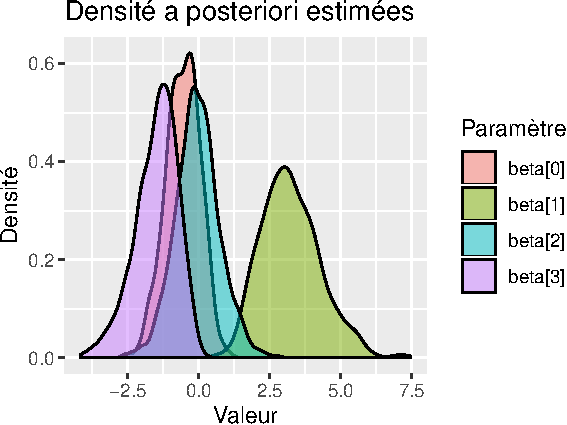
\includegraphics{correction_simulation_variables_aleatoires_files/figure-latex/accepted_samples-1} \end{center}

\begin{Shaded}
\begin{Highlighting}[]
\CommentTok{# Intervalle de confiance a posteriori pour la moyenne}
\NormalTok{accepted_samples }\OperatorTok\StringTok{ }
\StringTok{  }\KeywordTok{group_by}\NormalTok{(parameter) }\OperatorTok\StringTok{ }
\StringTok{  }\KeywordTok{summarise}\NormalTok{(}\DataTypeTok{ic_95_inf =} \KeywordTok{mean}\NormalTok{(value) }\OperatorTok{-}\StringTok{ }\FloatTok{1.96} \OperatorTok{*}\StringTok{ }\KeywordTok{sqrt}\NormalTok{(}\KeywordTok{var}\NormalTok{(value) }\OperatorTok{/}\StringTok{ }\KeywordTok{n}\NormalTok{()),}
            \DataTypeTok{posterior_mean =} \KeywordTok{mean}\NormalTok{(value),}
            \DataTypeTok{ic_95_sup =} \KeywordTok{mean}\NormalTok{(value) }\OperatorTok{+}\StringTok{ }\FloatTok{1.96} \OperatorTok{*}\StringTok{ }\KeywordTok{sqrt}\NormalTok{(}\KeywordTok{var}\NormalTok{(value) }\OperatorTok{/}\StringTok{ }\KeywordTok{n}\NormalTok{()))}
\end{Highlighting}
\end{Shaded}

\begin{verbatim}
# A tibble: 4 x 4
  parameter ic_95_inf posterior_mean ic_95_sup
  <chr>         <dbl>          <dbl>     <dbl>
1 beta[0]     -0.597         -0.560   -0.523  
2 beta[1]      3.18           3.24     3.30   
3 beta[2]     -0.0941        -0.0459   0.00219
4 beta[3]     -1.55          -1.50    -1.45   
\end{verbatim}

\begin{enumerate}
\def\labelenumi{\arabic{enumi}.}
\setcounter{enumi}{8}
\tightlist
\item
  À partir de cette méthode, et en utilisant les questions 3 et 4,
  donner une estimation ainsi qu'un intervalle de confiance pour à 95\%
  de la quantité
  \[\int_{\mathbb{R}^4}\pi(\theta)L(y_{1:n}\theta) \text{d} \theta\]
\end{enumerate}

\begin{Correction}
Il suffit simplement d'implémenter les formules vues plus haut. À partir du tableau des candidats, on peut extraire les temps d'attente observés.
On note \texttt{I\_hat} la quantité recherchée
\end{Correction}

\begin{Shaded}
\begin{Highlighting}[]
\NormalTok{nb_essais <-}\StringTok{ }\NormalTok{acceptance_reject_candidates }\OperatorTok\StringTok{ }
\StringTok{  }\KeywordTok{group_by}\NormalTok{(Replicate) }\OperatorTok\StringTok{ }
\StringTok{  }\KeywordTok{summarise}\NormalTok{(}\DataTypeTok{nb_essai =} \KeywordTok{n}\NormalTok{()) }\OperatorTok\StringTok{ }
\StringTok{  }\KeywordTok{pull}\NormalTok{(nb_essai)}
\NormalTok{tau_hat <-}\StringTok{ }\KeywordTok{mean}\NormalTok{(nb_essais)}
\NormalTok{I_hat <-}\StringTok{ }\NormalTok{M_tilde }\OperatorTok{/}\StringTok{ }\NormalTok{tau_hat }\CommentTok{# Estimation}
\NormalTok{S_square <-}\StringTok{ }\KeywordTok{var}\NormalTok{(nb_essais)}
\CommentTok{# Intervalle de confiance}
\NormalTok{(IC_}\DecValTok{95}\NormalTok{_I_hat <-}\StringTok{ }\NormalTok{I_hat }\OperatorTok{+}\StringTok{ }\KeywordTok{c}\NormalTok{(}\OperatorTok{-}\DecValTok{1}\NormalTok{, }\DecValTok{1}\NormalTok{) }\OperatorTok{*}\StringTok{ }\KeywordTok{qnorm}\NormalTok{(}\FloatTok{0.975}\NormalTok{) }\OperatorTok{*}\StringTok{ }\NormalTok{M_tilde }\OperatorTok{/}\StringTok{ }\NormalTok{tau_hat}\OperatorTok{^}\DecValTok{2} \OperatorTok{*}\StringTok{ }\KeywordTok{sqrt}\NormalTok{(S_square }\OperatorTok{/}\StringTok{ }\NormalTok{n_samples))}
\end{Highlighting}
\end{Shaded}

\begin{verbatim}
[1] 3.688814e-05 4.150727e-05
\end{verbatim}

\begin{enumerate}
\def\labelenumi{\arabic{enumi}.}
\setcounter{enumi}{9}
\tightlist
\item
  Afin d'estimer \(\mathbb{E}[\theta \vert y_{1:n}]\), implémenter
  l'estimateur \(\hat{J}_N\) de la question 6 (avec le même algorithme
  d'acceptation rejet que pour la question 8). Donnez un intervalle de
  confiance asymptotique pour l'estimation obtenue.
\end{enumerate}

\begin{Correction}
À $M$ connu, la réponse est un application directe de la section précédente. Malheureusement, ici, on ne connait que $\tilde{M}$. Par l'exercice précédent (pour une densité cible $f$ connue seulement au travers de $\tilde{f}$), on sait que pour chaque $\tilde{M}$ valable, correspond un $M = \frac{\tilde{M}}{I(\tilde{f})}$. Dans ce cas, effectuer l'acceptation rejet avec $f$, $g$ et $M$ est équivalent (en terme de probabilité d'acceptation) qu'effectuer l'acceptation rejet avec $\tilde{f}$, $g$. Il suffit donc de remplacer M par $\tilde{M} / I(\tilde{f})$ dans la formule et tout doit fonctionner.

Malheureusement $I(\tilde{f})$ est inconnue.
En remplaçant $\tilde{M} / I(\tilde{f})$ par son estimateur Monte Carlo naturel qui est $\hat{M} = \frac{\tilde{M}}{\hat{I}_n(\tilde{f})} = \frac{N}{n}$, on obtient l'estimateur 
$$\tilde{J}_n = \frac{1}{N} \left(\sum_{i = 1}^n \varphi(X_i) + (\frac{N}{n} - 1) \sum_{j = 1}^{N - n} \frac{\tilde{f}(Z_j)}{\tilde{M}g(Z_j) - \tilde{f} (Z_j)}\varphi(Z_j) \right)$$

Cet estimateur est désormais biaisé, mais consistant.
Montrer cette consistance n'est pas trivial et cela dépasse le cadre de l'exercice (et de ce cours), donc on l'admettra. De même, la variance asymptotique de cet estimateur ne va pouvoir s'exprimer facilement ici.

Je n'avais pas vu ce détail en rédigeant le sujet, je ne noterai donc pas cette question.
Je tiens à 'excuser auprès de celles et ceux qui se seraient arracher les cheveux là dessus. Celles et ceux ayant eu des idées pertinentes auront un bonus (notamment, de remplacer $M$ par son estimateur). Les étudiant(e)s intéressés pour approfondir pourront lire l'article de référence: \textit{Post-Processing Accept-Reject Samples: Recycling and Rescaling} de G. Casella et C. Robert (1998).

Toujours est il que cet estimateur est implémentable facielement.
\end{Correction}

\begin{Shaded}
\begin{Highlighting}[]
\CommentTok{# Fonctions g, f, et de calcul des poids d'importances}
\NormalTok{get_g <-}\StringTok{ }\ControlFlowTok{function}\NormalTok{(beta_vec)\{}
  \KeywordTok{prod}\NormalTok{(}\KeywordTok{dnorm}\NormalTok{(beta_vec, }\DecValTok{0}\NormalTok{, }\DecValTok{2}\NormalTok{))}
\NormalTok{\}}
\NormalTok{get_f <-}\StringTok{ }\ControlFlowTok{function}\NormalTok{(beta_vec)\{}
  \KeywordTok{get_g}\NormalTok{(beta_vec) }\OperatorTok{*}\StringTok{ }\KeywordTok{get_likelihood}\NormalTok{(beta_vec, design_matrix, y_vector)}
\NormalTok{\}}
\NormalTok{get_is_weight <-}\StringTok{ }\ControlFlowTok{function}\NormalTok{(beta_vec, M_estimate, M_tilde,}
                          \DataTypeTok{accepted =} \OtherTok{FALSE}\NormalTok{)\{}
  \ControlFlowTok{if}\NormalTok{(}\OperatorTok{!}\NormalTok{accepted)\{}
\NormalTok{    f_beta <-}\StringTok{ }\KeywordTok{get_f}\NormalTok{(beta_vec)}
    \KeywordTok{return}\NormalTok{((M_estimate }\OperatorTok{-}\StringTok{ }\DecValTok{1}\NormalTok{) }\OperatorTok{*}\StringTok{ }\NormalTok{f_beta }\OperatorTok{/}\StringTok{ }
\StringTok{             }\NormalTok{(M_tilde }\OperatorTok{*}\StringTok{ }\KeywordTok{get_g}\NormalTok{(beta_vec) }\OperatorTok{-}\StringTok{ }\NormalTok{f_beta))}
\NormalTok{  \}}
  \ControlFlowTok{else}
    \KeywordTok{return}\NormalTok{(}\DecValTok{1}\NormalTok{)}
\NormalTok{\}}
\end{Highlighting}
\end{Shaded}

\begin{Shaded}
\begin{Highlighting}[]
\CommentTok{# Ici, un peu de préparation de donnees}
\CommentTok{# On cree un tableau ayant en colonne les argiments nécessaires}
\NormalTok{arguments_tibble <-}\StringTok{ }
\StringTok{  }\NormalTok{acceptance_reject_candidates }\OperatorTok\StringTok{ }
\StringTok{  }\KeywordTok{select}\NormalTok{(}\OperatorTok{-}\NormalTok{Replicate) }\OperatorTok\StringTok{ }
\StringTok{  }\KeywordTok{rowid_to_column}\NormalTok{(}\DataTypeTok{var =} \StringTok{"index"}\NormalTok{) }\OperatorTok\StringTok{ }
\StringTok{  }\KeywordTok{nest}\NormalTok{(}\DataTypeTok{beta_vec =} \KeywordTok{c}\NormalTok{(beta_}\DecValTok{0}\NormalTok{, beta_}\DecValTok{1}\NormalTok{, beta_}\DecValTok{2}\NormalTok{, beta_}\DecValTok{3}\NormalTok{)) }\OperatorTok\StringTok{ }
\StringTok{  }\KeywordTok{mutate}\NormalTok{(}\DataTypeTok{beta_vec =} \KeywordTok{map}\NormalTok{(beta_vec, }\ControlFlowTok{function}\NormalTok{(x) }\KeywordTok{as.numeric}\NormalTok{(x))) }\OperatorTok\StringTok{ }
\StringTok{  }\KeywordTok{select}\NormalTok{(}\OperatorTok{-}\NormalTok{index)}
\CommentTok{# Maintenant, on cree le bon tableau}
\NormalTok{estimates_recyling_ar <-}\StringTok{ }\NormalTok{acceptance_reject_candidates }\OperatorTok\StringTok{ }
\StringTok{  }\KeywordTok{mutate}\NormalTok{(}\DataTypeTok{is_weights =} \KeywordTok{pmap_dbl}\NormalTok{(}\DataTypeTok{.l =}\NormalTok{ arguments_tibble, }\DataTypeTok{.f =}\NormalTok{ get_is_weight, }
                               \DataTypeTok{M_estimate =}\NormalTok{ tau_hat, }\DataTypeTok{M_tilde =}\NormalTok{ M_tilde)) }\OperatorTok\StringTok{ }
\StringTok{  }\KeywordTok{mutate}\NormalTok{(}\DataTypeTok{iteration =} \DecValTok{1}\OperatorTok{:}\KeywordTok{n}\NormalTok{()) }\OperatorTok\StringTok{ }
\StringTok{  }\KeywordTok{mutate_at}\NormalTok{(}\DataTypeTok{.vars =} \KeywordTok{vars}\NormalTok{(}\KeywordTok{starts_with}\NormalTok{(}\StringTok{"beta_"}\NormalTok{)), }
            \DataTypeTok{.funs =} \ControlFlowTok{function}\NormalTok{(colonne) }\KeywordTok{cumsum}\NormalTok{(colonne }\OperatorTok{*}\StringTok{ }\NormalTok{.}\OperatorTok{$}\NormalTok{is_weights) }\OperatorTok{/}\StringTok{ }\NormalTok{.}\OperatorTok{$}\NormalTok{iteration) }\OperatorTok\StringTok{ }
\StringTok{  }\KeywordTok{mutate}\NormalTok{(}\DataTypeTok{methode =} \StringTok{"AR + Recyclage"}\NormalTok{) }\OperatorTok\StringTok{ }
\StringTok{  }\KeywordTok{select}\NormalTok{(}\OperatorTok{-}\NormalTok{Replicate, }\OperatorTok{-}\NormalTok{accepted, }\OperatorTok{-}\NormalTok{is_weights) }\OperatorTok
\StringTok{  }\KeywordTok{slice}\NormalTok{(}\KeywordTok{seq}\NormalTok{(}\DecValTok{1}\NormalTok{, }\KeywordTok{n}\NormalTok{(), }\DataTypeTok{by =} \DecValTok{100}\NormalTok{)) }\OperatorTok\StringTok{ }\CommentTok{# Only kepp one point in 100}
\StringTok{  }\KeywordTok{gather}\NormalTok{(}\OperatorTok{-}\NormalTok{iteration, }\OperatorTok{-}\NormalTok{methode, }\DataTypeTok{key =} \StringTok{"Parametre"}\NormalTok{, }\DataTypeTok{value =} \StringTok{"value"}\NormalTok{)}
\end{Highlighting}
\end{Shaded}

\begin{Shaded}
\begin{Highlighting}[]
\NormalTok{estimates_classic_ar <-}\StringTok{ }\NormalTok{acceptance_reject_candidates }\OperatorTok\StringTok{ }
\StringTok{  }\KeywordTok{filter}\NormalTok{(accepted) }\OperatorTok\StringTok{ }
\StringTok{  }\KeywordTok{mutate}\NormalTok{(}\DataTypeTok{iteration =} \DecValTok{1}\OperatorTok{:}\KeywordTok{n}\NormalTok{()) }\OperatorTok\StringTok{ }
\StringTok{  }\KeywordTok{mutate_at}\NormalTok{(}\DataTypeTok{.vars =} \KeywordTok{vars}\NormalTok{(}\KeywordTok{starts_with}\NormalTok{(}\StringTok{"beta_"}\NormalTok{)), }
            \DataTypeTok{.funs =} \ControlFlowTok{function}\NormalTok{(colonne) }\KeywordTok{cumsum}\NormalTok{(colonne) }\OperatorTok{/}\StringTok{ }\NormalTok{.}\OperatorTok{$}\NormalTok{iteration) }\OperatorTok\StringTok{ }
\StringTok{  }\KeywordTok{mutate}\NormalTok{(}\DataTypeTok{methode =} \StringTok{"AR classique"}\NormalTok{) }\OperatorTok\StringTok{ }
\StringTok{  }\KeywordTok{select}\NormalTok{(}\OperatorTok{-}\NormalTok{Replicate, }\OperatorTok{-}\NormalTok{accepted) }\OperatorTok
\StringTok{  }\KeywordTok{gather}\NormalTok{(}\OperatorTok{-}\NormalTok{iteration, }\OperatorTok{-}\NormalTok{methode, }\DataTypeTok{key =} \StringTok{"Parametre"}\NormalTok{, }\DataTypeTok{value =} \StringTok{"value"}\NormalTok{)}
\CommentTok{# On crée une colonne de poids, valant 1 si l'échantillon a été accetpé,}
\CommentTok{# donnée par get_is_weight sinon}
\end{Highlighting}
\end{Shaded}

\begin{enumerate}
\def\labelenumi{\arabic{enumi}.}
\setcounter{enumi}{10}
\tightlist
\item
  Comparez les deux estimateurs et commentez.
\end{enumerate}

\begin{Correction}
Pour un $\hat{M}$ fixé, on trace les réalisation des estimateurs au cours des itérations.
On constate que la variance de l'estimateur avec recyclage est bien plus forte (et on ne prend pas en compte ici la variance de $\hat{M}$)! On voit que cette variance est bien plus forte même si le nombre d'échantillons total est beaucoup plus grand.

On peut ainsi voir ici qu'inclure tous les échantillons peut venir au prix d'une variance plus forte. L'idée du recyclage, séduisante en théorie, n'est pas toujours bonne en pratique.
\end{Correction}

\begin{Shaded}
\begin{Highlighting}[]
\KeywordTok{bind_rows}\NormalTok{(estimates_recyling_ar, }
\NormalTok{          estimates_classic_ar) }\OperatorTok\StringTok{ }
\StringTok{  }\KeywordTok{ggplot}\NormalTok{(}\KeywordTok{aes}\NormalTok{(}\DataTypeTok{x =}\NormalTok{ iteration, }\DataTypeTok{y =}\NormalTok{ value)) }\OperatorTok{+}
\StringTok{  }\KeywordTok{geom_path}\NormalTok{(}\KeywordTok{aes}\NormalTok{(}\DataTypeTok{color =}\NormalTok{ Parametre)) }\OperatorTok{+}
\StringTok{  }\KeywordTok{facet_wrap}\NormalTok{(.}\OperatorTok{~}\NormalTok{methode, }\DataTypeTok{scales =} \StringTok{"free_x"}\NormalTok{) }\OperatorTok{+}
\StringTok{  }\KeywordTok{theme}\NormalTok{(}\DataTypeTok{axis.text =} \KeywordTok{element_text}\NormalTok{(}\DataTypeTok{angle =} \DecValTok{45}\NormalTok{)) }\OperatorTok{+}
\StringTok{  }\KeywordTok{labs}\NormalTok{(}\DataTypeTok{x =} \StringTok{"Iteration"}\NormalTok{, }\DataTypeTok{y =} \StringTok{"Valeur estimée"}\NormalTok{,}
       \DataTypeTok{title =} \StringTok{"Estimation de l'espérance a posteriori"}\NormalTok{)}
\end{Highlighting}
\end{Shaded}

\begin{center}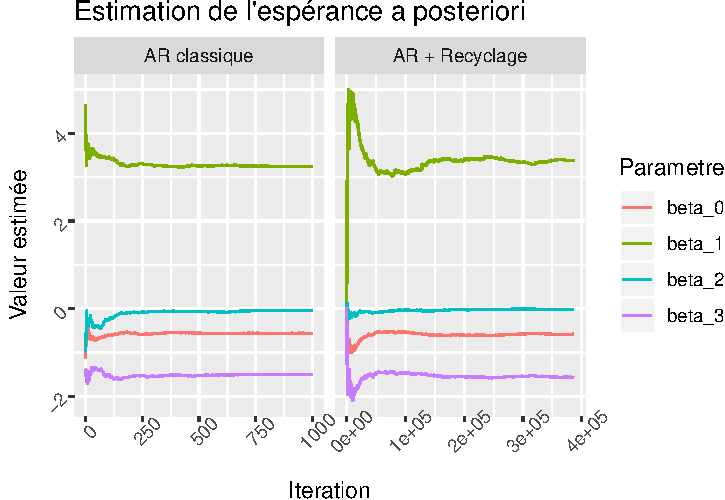
\includegraphics{correction_simulation_variables_aleatoires_files/figure-latex/comparaison_estimateur_esperances-1} \end{center}


\end{document}
